\chapter{Program Creation} % (fold)
\label{cha:program_creation}

\begin{quote}
  \Fontlukas\Large
  \renewcommand{\LettrineTextFont}{\relax}
  \lettrine[image=true,lines=3,lraise=0.1]
  {C}{asting} spells crafted by others is alright, but the true power of magic can only be realised by crafting your own spells. You have done well mastering the tools, so now let us turn our attention to the study of the arcane knowledge of spell craft. To create your own spells you need to know\ldots
\end{quote}

\bigskip

Compiling programs crafted by others is alright, but the true power of programming can only be realised by learning to craft your own programs. \cref{cha:building programs} introduced you to the tools you need to compile programs from source code, so now we can turn our attention to the study program creation.

This chapter introduces the artefacts used to create programs, and how you can code these using a programming language. You will start by learning to create simple programs that output information to the Terminal.

When you have understood the material in this chapter you will be able to write the code needed to declare a program, convert this code into an executable program using a compiler, and then run the program you created. You will have made those first important steps in your journey to master this arcane knowledge. 

\minitoc

% ============
% = Concepts =
% ============
\clearpage
\section{Program Creation Concepts} % (fold)
\label{sec:program_creation_concepts}

Our first program is going to display some text to the Terminal. In this section you will be introduced to the programming artefacts and terminology you will need to use to create this program. This first step is important and will require you to have installed a C or Pascal compiler, see \cref{cha:building programs} for instructions.

A programming \textbf{artefact} is something that can be created and used within your code. In this chapter we will look at creating Programs, and using a number of other artefacts. The following artefacts will be covered in this chapter:
\begin{itemize}
  \item \nameref{sub:program}: You declare a Program to get the compiler to write a file that can be executed.
  \item \nameref{sub:procedure}: You can call Procedures to perform actions within the program.
  \item \nameref{sec:program-creation-library}: The program can use code from other Libraries. These libraries contain reusable Procedures and Types. 
  \item \nameref{sub:type}: A Type defines how data is interpreted by the program. The language will support a number of basic types by default, and Libraries can add other types. 
\end{itemize}

In addition to these artefacts, you will need to understand some programming \textbf{terminology}. The following terms are discussed in this section:
\begin{itemize}
  \item \nameref{sec:program-creation-statement}: An \textbf{instruction} within the Program.
  \item \nameref{sub:expression}: A \textbf{value} used in a Statement.
  \item \nameref{sub:identifier}: The \textbf{name} of an artefact.
  % \item Literal: A part of an \textbf{expression} where the value is entered directly into the code.
\end{itemize}

This section also introduces the following kinds of instructions. You can use these to get the computer to perform certain \textbf{actions} within your program.
\begin{itemize}
  \item \nameref{sub:procedure call}: The instruction to run a Procedure.
\end{itemize}

We can then use these concepts, artefacts, and instructions to create a Program that includes a call to a procedure that will write some text to the Terminal as shown in Figure \ref{fig:program-creation-helloworld}.

\begin{figure}[h]
   \centering
   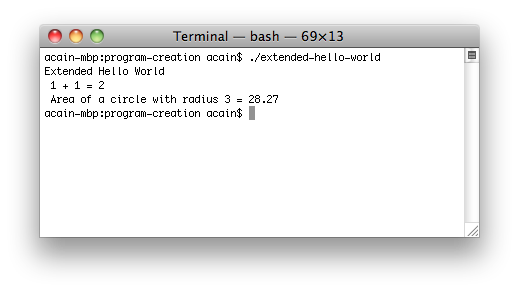
\includegraphics[width=0.8\textwidth]{./topics/program-creation/images/HelloWorld} 
   \caption[Hello World Terminal]{Hello World run from the Terminal}
   \label{fig:program-creation-helloworld}
\end{figure}

\clearpage
\subsection{Program} % (fold)
\label{sub:program}

A program contains the instructions the computer will follow when that program is executed. In your source code you can declare a program in which you code the steps you want followed when your program is executed. When you compile this code the compiler will create an executable file (a \emph{program}) that the user can run. Running the program will then get the computer to perform the steps you wrote in the code.

\begin{figure}[h]
   \centering
   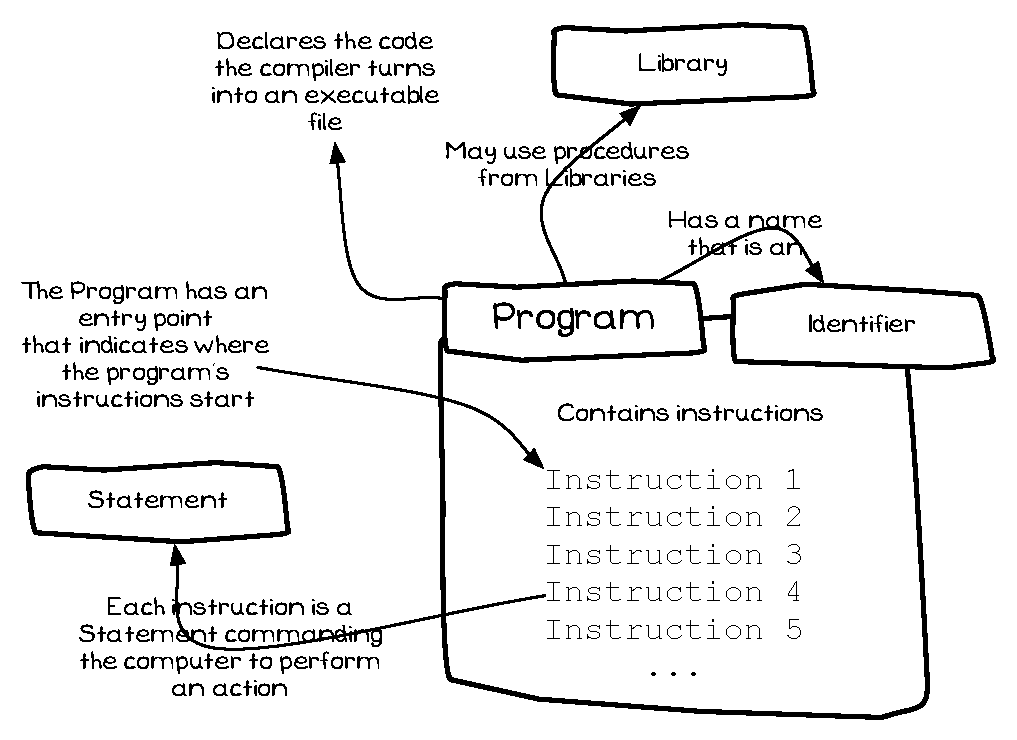
\includegraphics[width=\textwidth]{./topics/program-creation/diagrams/BasicProgramConcept} 
   \caption{A program contains instructions that command the computer to perform actions}
   \label{fig:program-creation-program}
\end{figure}


\mynote{
\begin{itemize}
  \item A program is an \textbf{artefact}, something you can create in your code.
  \item Figure \ref{fig:program-creation-program} shows the concepts related to programs.
  \item A program is a programming artefact used to define the steps to perform when the program is run.
  \item You use the compiler to convert the program's source code into an executable file.
  \item By declaring a program in your code you are telling the compiler to create a file the user can run.
  \item The program has an \textbf{entry point} that indicates where the program's instructions start.
  \item The name of the program determines the name of the executable file.
  \item Your program can use code from a \nameref{sub:library} or number of libraries.
  \item In programming terminology, an instruction is called a \nameref{sub:statement}.
\end{itemize}
}

% section program (end)
\clearpage
\subsection{Statement} % (fold)
\label{sub:statement}

A statement is an instruction for the computer to perform an action, a command telling it what to do. Each \nameref{sub:program} contains a list of statements (commands). When the program is run the computer follows these commands one at a time, in sequence, starting at the program's entry point and ending when it completes the program's last statement.

\begin{figure}[h]
   \centering
   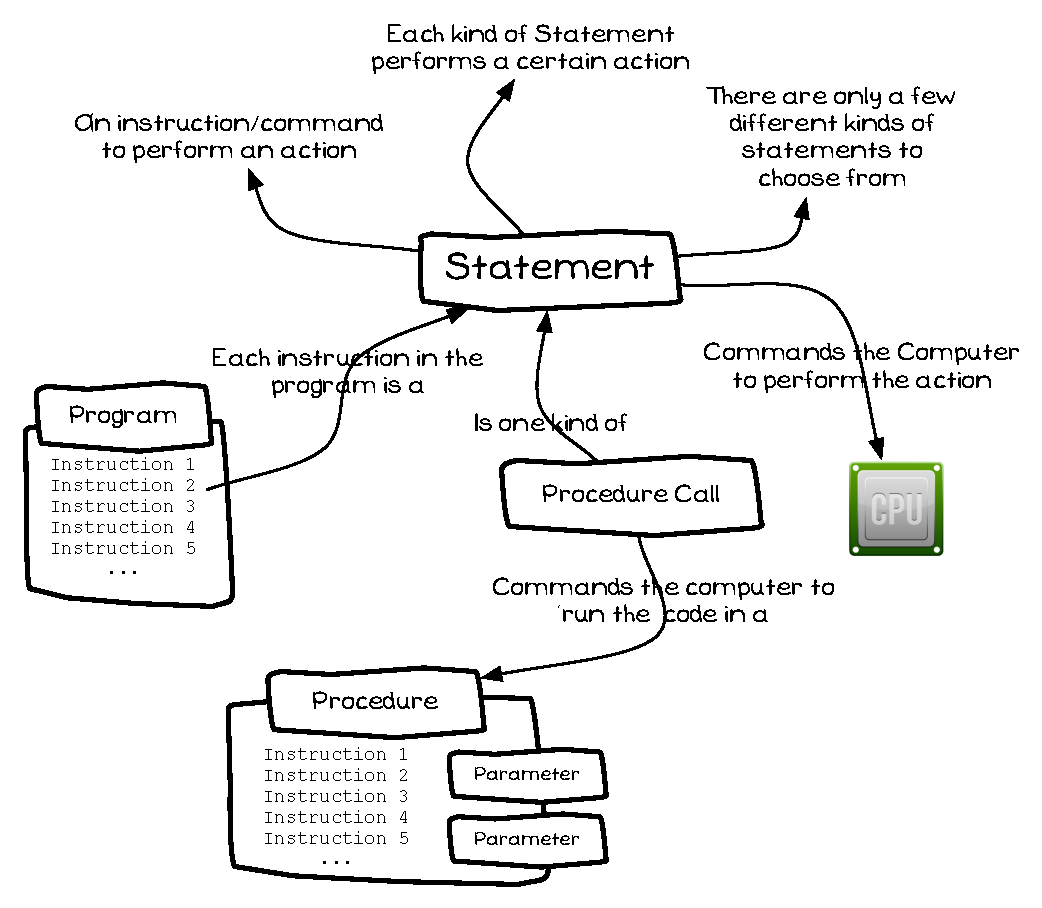
\includegraphics[width=\textwidth]{./topics/program-creation/diagrams/Statement} 
   \caption{A statement is a command for the computer to perform an action}
   \label{fig:program-creation-statement}
\end{figure}


\mynote{
\begin{itemize}
  \item A statement is a \textbf{term} used to describe the instructions in your code.
  \item Figure \ref{fig:program-creation-statement} shows the concepts related to statements.
  \item A statement is a \textbf{command}, an instruction to perform a task.
  \item A \nameref{sub:program} has a list of statements that are followed when it is executed.
  \item There are only a few different kinds of statement.
  \item A \nameref{sub:procedure call} is a kind of statement, it tells the computer to run the code in a \nameref{sub:procedure}.
  \item This style of programming is known as \textbf{Imperative} programming. Imperative means to give authoritative commands, and that is what we do in our programs. Our programs are lists of authoritative commands telling the computer to perform actions.
\end{itemize}
}

% section statement (end)
\clearpage
\subsection{Procedure Call} % (fold)
\label{sub:procedure call}

A procedure call is a kind of \nameref{sub:statement} that instructs the computer to run the code in a \nameref{sub:procedure}. If the procedure requires some data to work with, then this data is passed to the procedure as part of the procedure call. The procedure's name is used to identify the procedure to call.

\begin{figure}[h]
   \centering
   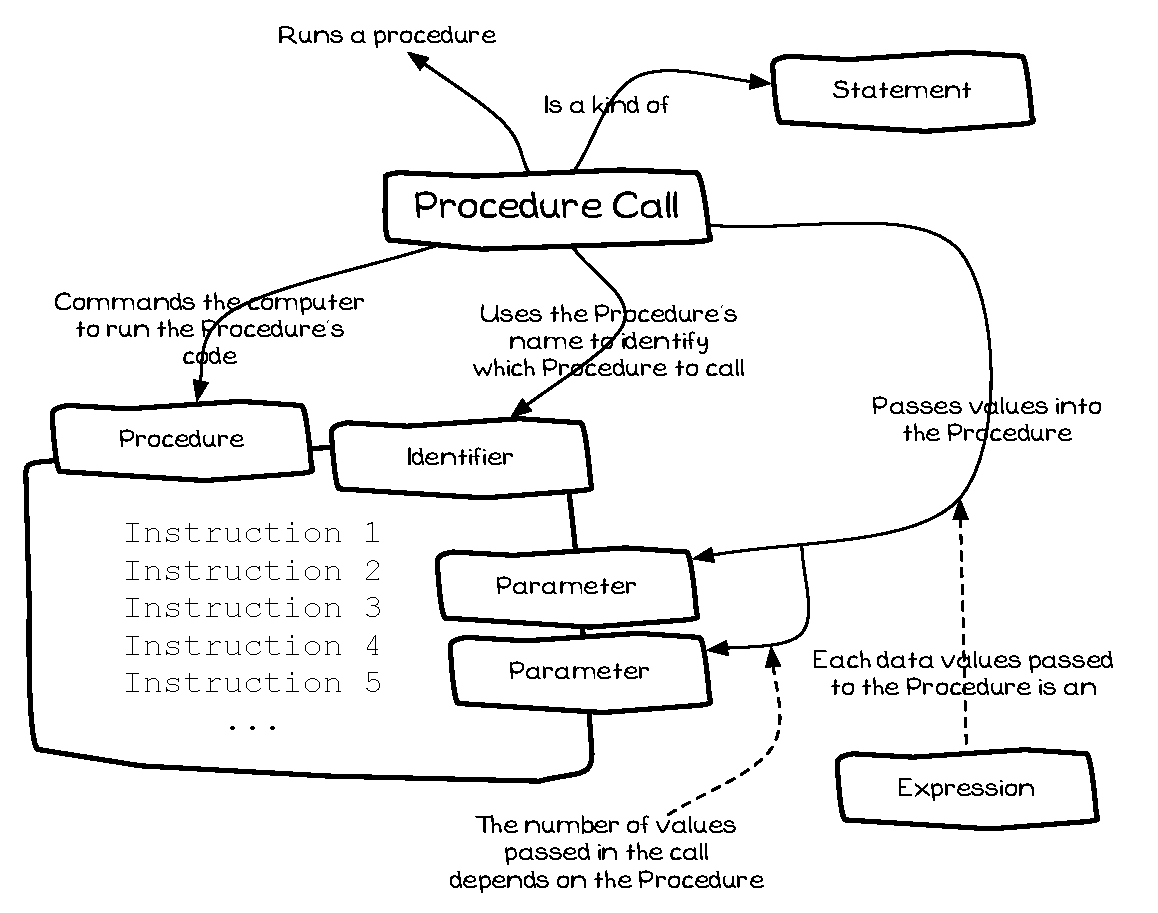
\includegraphics[width=\textwidth]{./topics/program-creation/diagrams/ProcedureCall} 
   \caption{A procedure calls runs a procedure, passing in values for the procedure to use}
   \label{fig:program-creation-procedure call}
\end{figure}


\mynote{
\begin{itemize}
  \item A procedure call is an \textbf{action}, you can call procedures in your code.
  \item Figure \ref{fig:program-creation-procedure call} shows the concepts related to the procedure call.
  \item A procedure call is an instruction to execute a procedure.
  \item You can code a procedure anywhere you can code a statement.
  \item The \nameref{sub:identifier} indicates the \nameref{sub:procedure} to call.
  \item Data values passed to the procedure are coded using \nameref{sub:expression}s.
  \item When the procedure's task is complete the program continues with the next \nameref{sub:statement}.
\end{itemize}
}

% section program (end)
\clearpage
\subsection{Procedure} % (fold)
\label{sub:procedure}

A Procedure is a part of a \nameref{sub:program} that performs a specific task. Each Procedure has a name that should reflect the task the procedure carries out. When a Procedure is called it gets control of the computer and instructs it to perform the steps needed to carry out the task the Procedure is responsible for. Often these tasks require data, so the Procedure may need to be passed data when it is called. When the procedure finishes its task control returns back to the code that called the Procedure.

\begin{figure}[h]
   \centering
   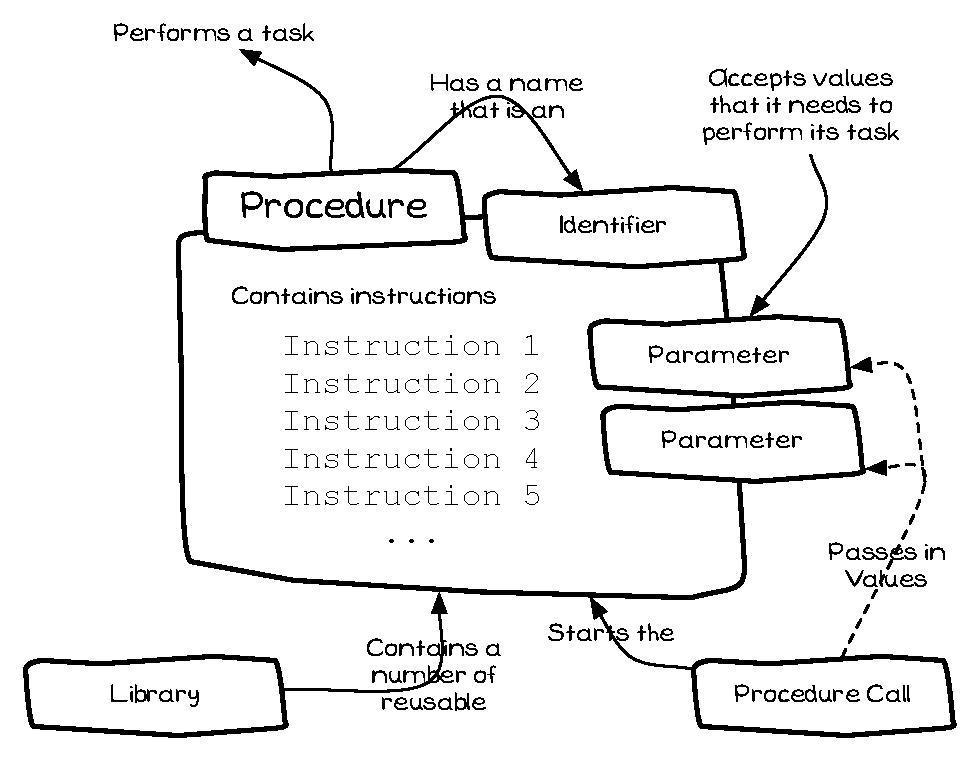
\includegraphics[width=\textwidth]{./topics/program-creation/diagrams/Procedure} 
   \caption[Procedure Concept Diagram]{A Procedure contains instructions to perform a task, and may need to be passed data in order to do this}
   \label{fig:program-creation-procedure}
\end{figure}


\mynote{
\begin{itemize}
  \item Figure \ref{fig:program-creation-procedure} shows the concepts related to Procedures.
  \item A Procedure is a programming artefact that can be called to perform a certain task.
  \item The name of a Procedure is an \nameref{sec:program-creation-identifier}.
  \item Each \nameref{sec:program-creation-library} will contain a number of Procedures to perform common tasks.
  \item The standard library will include procedures to write values to the console.
  \item The SwinGame libraries contain procedures that can draw images on the screen, play sounds, and perform other tasks needed to create small games.
  \item Procedures are also called \textbf{subroutines}, \textbf{sub programs}, \textbf{methods} or \textbf{sub procedures}.
\end{itemize}
}

% section program (end)
\clearpage
\subsection{Expression} % (fold)
\label{sub:expression}

An Expression is a value used in a \nameref{sec:program-creation-statement}. These values may be calculated or entered directly into the source code of the Program.

\begin{figure}[h]
   \centering
   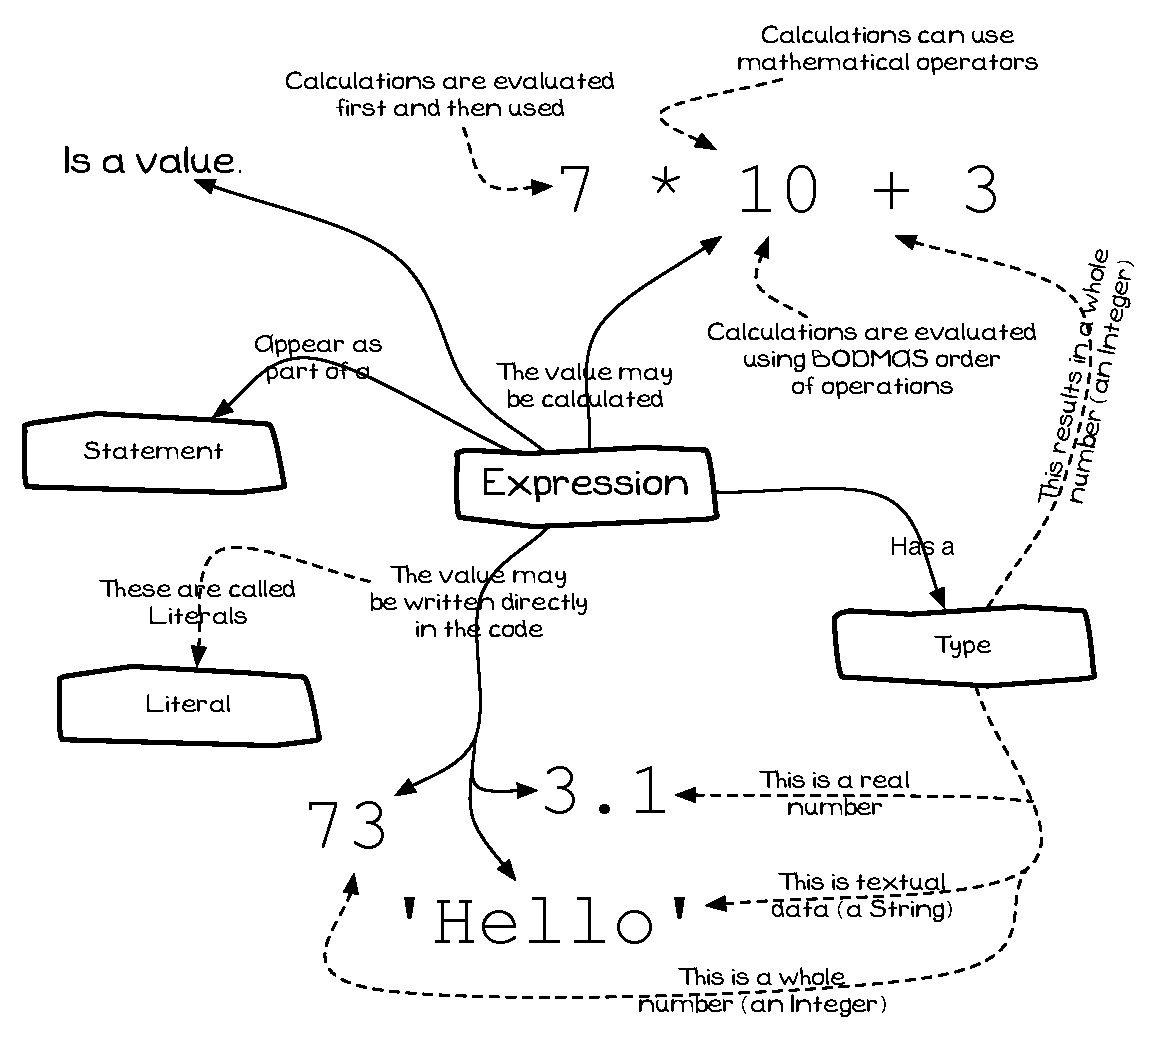
\includegraphics[width=\textwidth]{./topics/program-creation/diagrams/Expression} 
   \caption[Expression Concept Diagram]{An Expression provides a \textbf{value} to be used in a Statement.}
   \label{fig:program-creation-expression}
\end{figure}


\mynote{
\begin{itemize}
  \item The concepts related to Expressions are shown in Figure \ref{fig:program-creation-expression}.
  \item An Expression provides a \textbf{value} that is used in a Statement.
  \item The Expression's value may be calculated or entered directly into the code.
  \item Calculations can use mathematical operators: + for addition, - for subtraction, * for multiplication, $/$ for division, and parenthesis ( ) for grouping.
  \item Expressions are evaluated using the BODMAS order of operations.
  \item Values entered directly within an Expression are \textbf{Literal} values.
\end{itemize}
}

% section program (end)
% \clearpage
\subsection{Literal} % (fold)
\label{sec:program-creation-literal}

A Literal is a whole, or part of, an \nameref{sub:expression} where the value is entered directly into the code.

\begin{figure}[h]
   \centering
   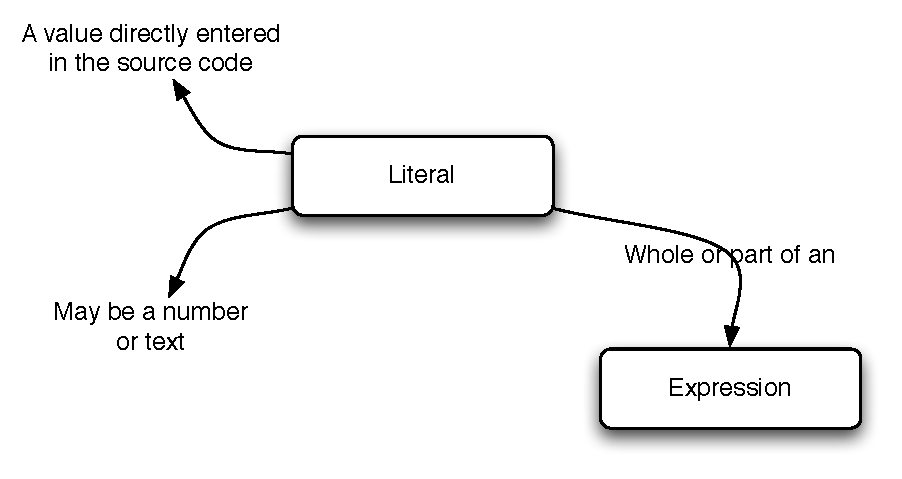
\includegraphics[width=0.8\textwidth]{./topics/program-creation/diagrams/Literal} 
   \caption[Literal Concept Diagram]{Concepts related to Literals.}
   \label{fig:program-creation-literal}
\end{figure}


\mynote{
\begin{itemize}
  \item Figure \ref{fig:program-creation-literal} shows the concepts relate to Literals.
  \item A Literal is a value entered directly into the program's source code.
  \item The value of a Literal can be a number or text.
  \item A Literal can be part or all of an \nameref{sub:expression}.
  \item These values are \emph{hard coded} into the program.
\end{itemize}
}

% section program (end)
\clearpage
\subsection{Type} % (fold)
\label{sub:type}

All values within a program will have a type. The type indicates how the data stored in the computers memory is interpreted by the program. There are three basic data types available in a programming language.

\begin{itemize}
    \item \textbf{Textual} data such as `\emph{Fred}', `\emph{Hello World}', `\emph{23}', and `\emph{This is text!}'.
    \item \textbf{Whole numbers} such as \emph{1}, \emph{0}, \emph{-5}, and \emph{37}.
    \item \textbf{Real numbers} such as \emph{0.5}, \emph{-126.0}, \emph{3.141516}, and \emph{23.981}.
\end{itemize}

\begin{figure}[h]
   \centering
   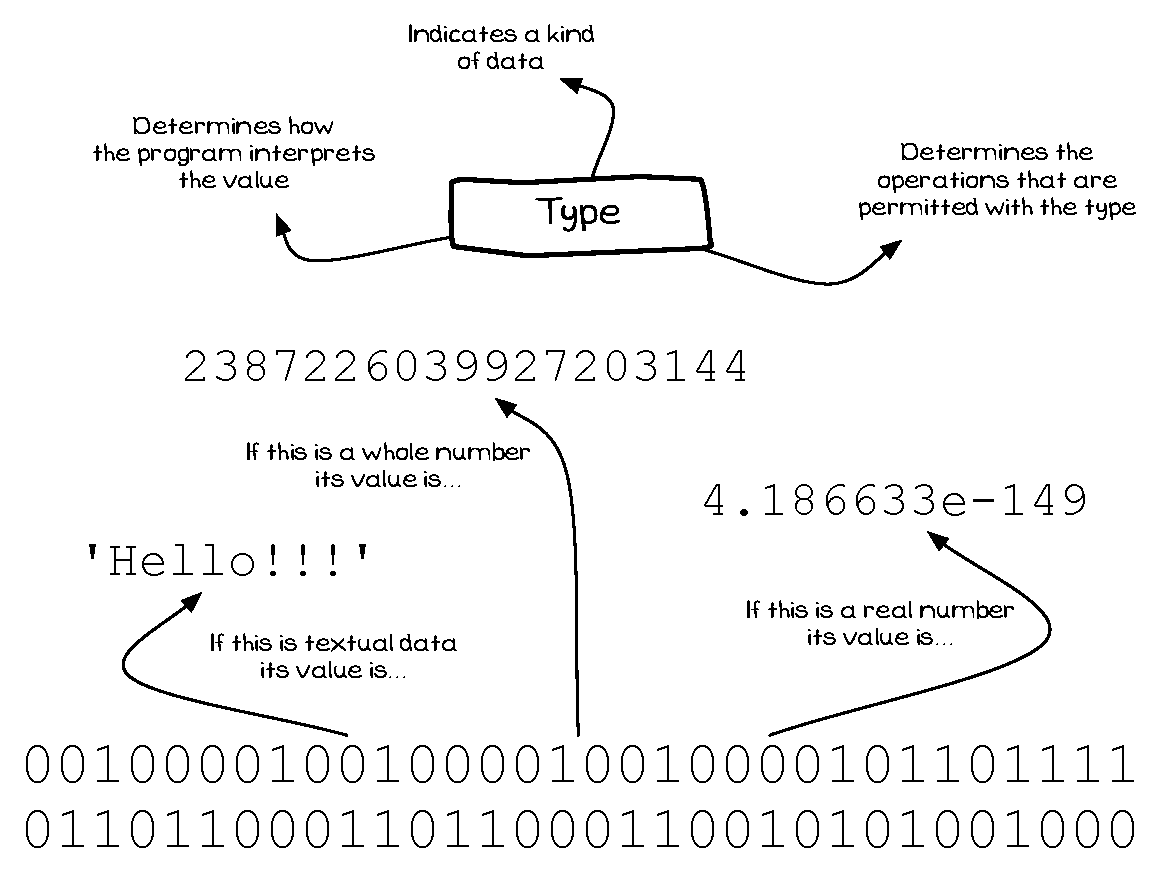
\includegraphics[width=0.95\textwidth]{./topics/program-creation/diagrams/Type} 
   \caption{Types defines how values are interpreted, and the operations that can be performed on the data}
   \label{fig:program-creation-type}
\end{figure}

\mynote{
\begin{itemize}
  \item A type is an \textbf{artefact}, there will be a number of existing types that you can use, and later you will see how to create your own types.
  \item The concepts related to expressions are shown in Figure \ref{fig:program-creation-type}.
  \item A type is a programming artefact that indicates a kind of data.
  \item The type determines the basic actions that can be performed on the value.
  \item The type determines the amount of memory needed to store a value of that kind.
  \item Whole numbers are usually called \textbf{Integers}.
  \item Real numbers are usually represented as \textbf{Floating Point} values. These values have a limited precision, supporting only a certain number of digits of precision.
  \item Textual values can contain numbers. In these cases the number are just textual representations of the values. For example, the text `\emph{23}' is the character `\emph{2}' followed by the character `\emph{3}', it is not the number \emph{23}.
  \item You can perform mathematic operations on numeric data, but not on textual data.
\end{itemize}
}

% section program (end)
\clearpage
\subsection{Identifier} % (fold)
\label{sub:identifier}

An Identifier is the technical term for the words that \emph{identify} something for the compiler. These can be the \textbf{name} of a programming artefact such as a Program, Library, or Procedure, or the words that have special means for the compiler. You will use Identifiers to name the artefact you create, and to select the appropriate artefact when it is used.

\begin{figure}[h]
   \centering
   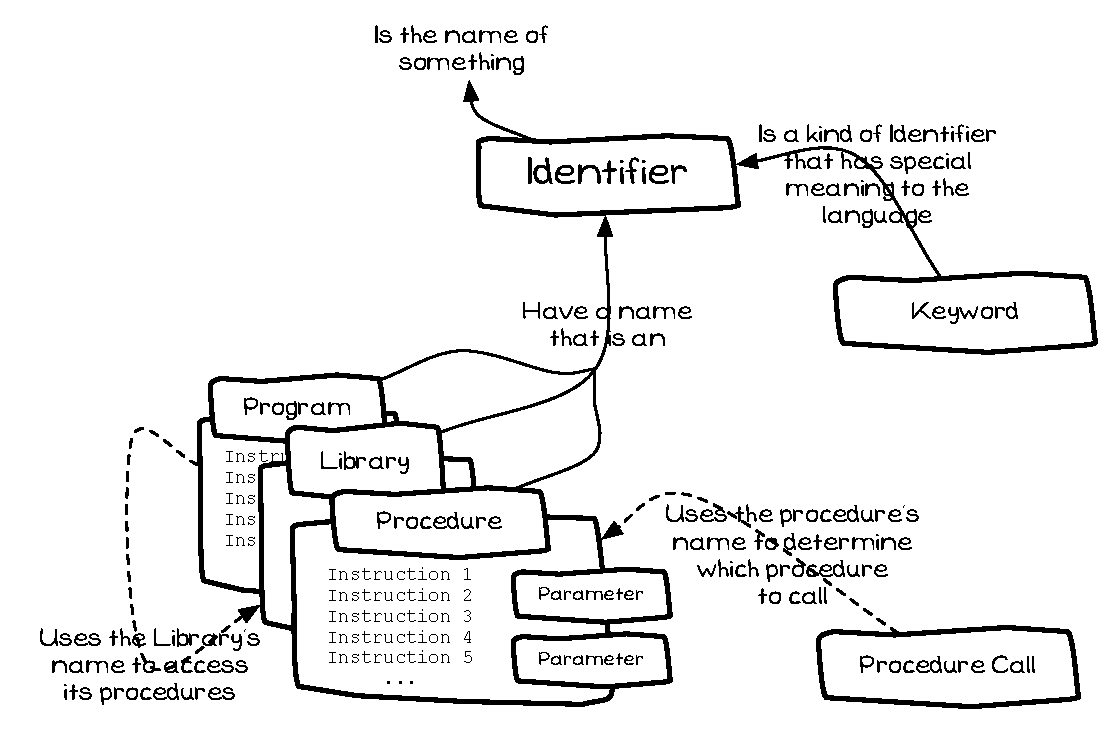
\includegraphics[width=\textwidth]{./topics/program-creation/diagrams/Identifier} 
   \caption[Identifier Concept Diagram]{An Identifier is the name of a programming artefact such as a Program, Library, or Procedure.}
   \label{fig:program-creation-identifier}
\end{figure}


\mynote{
\begin{itemize}
  \item Figure \ref{fig:program-creation-identifier} shows the concepts related to an Identifier.
  \item An Identifier is a \textbf{name} used to identify a programming artefact such as a \nameref{sub:program}, \nameref{sec:program-creation-library} or \nameref{sub:procedure}.
  \item The name you give your Program is an Identifier.
  \item You use Identifiers to indicate which Libraries you want to access in your Program.
  \item The \nameref{sub:procedure call} uses the Procedure's identifier to determine which procedure is called.
\end{itemize}
}

% section program (end)
\clearpage
\subsection{Library} % (fold)
\label{sec:program-creation-library}

A Library is a collection of reusable code artefacts. Each programming language has its own Library, and your programs can make use of the code available in this library.

\begin{figure}[h]
   \centering
   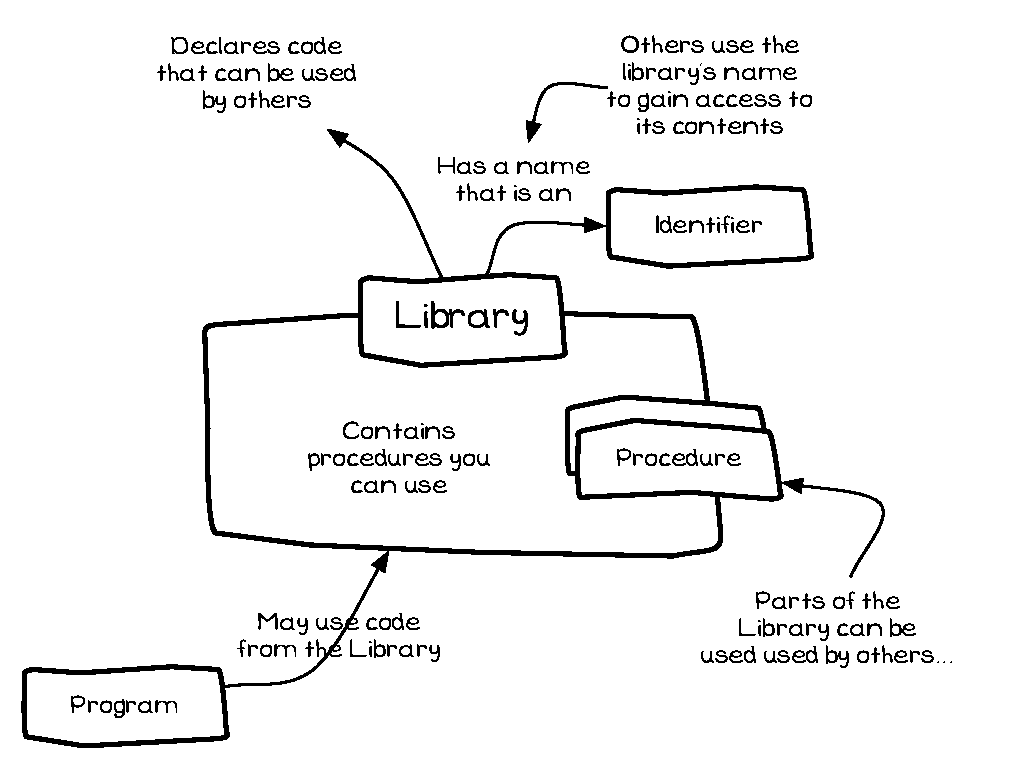
\includegraphics[width=\textwidth]{./topics/program-creation/diagrams/Library} 
   \caption[Library Concept Diagram]{A Library contains code that can be used by your Program}
   \label{fig:program-creation-library}
\end{figure}


\mynote{
\begin{itemize}
  \item Figure \ref{fig:program-creation-library} shows the concepts related to a Library.
  \item A Library is a collection of reusable code artefacts that you can use to perform certain tasks.
  \item The Library will contain \nameref{sub:procedure}s that perform a number of tasks.
  \item Each language has a standard library with code to perform many commonly performed tasks.
  \item Other libraries extend the capability of the languages further.
  \item SwinGame is a Library containing code to help you build games.
\end{itemize}
}

% section program (end)
\clearpage
\subsection{Comments} % (fold)
\label{sub:comments}

A program's source code contains instructions for the actions the computer must perform. However, this code is written and maintained by people. It is often useful to be able to place comments in the code to help someone reading that code understand how the code works or what it is trying to achieve. This text is not something that should be translated into machine code.

Programming languages include the ability to embed \emph{comments} that are ignored by the compiler when it compiles the code.

\bigskip

\mynote{
\begin{itemize}
  \item It is good practice to place a comment at the top of your code explaining what the program does.
  \item Comments should be included to help other people read your code. You will also find these comments useful when you return to your code after a long break.
  \item Make your comments meaningful, try to capture your intentions and ideas.
  \item Comments have no impact on the executable produced by the compiler.
\end{itemize}
}

% subsection comments (end)

% section program_creation_concepts (end)

\clearpage
\subsection{Summary} % (fold)
\label{sub:program_creation_concepts_summary}

This section has introduced a number of programming artefacts, some programming terminology, and one kind of instruction. An overview of these concepts is shown in Figure \ref{fig:program-creation-summary}. The next section will look at how you can use these concepts to design some small programs.

\begin{figure}[h]
   \centering
   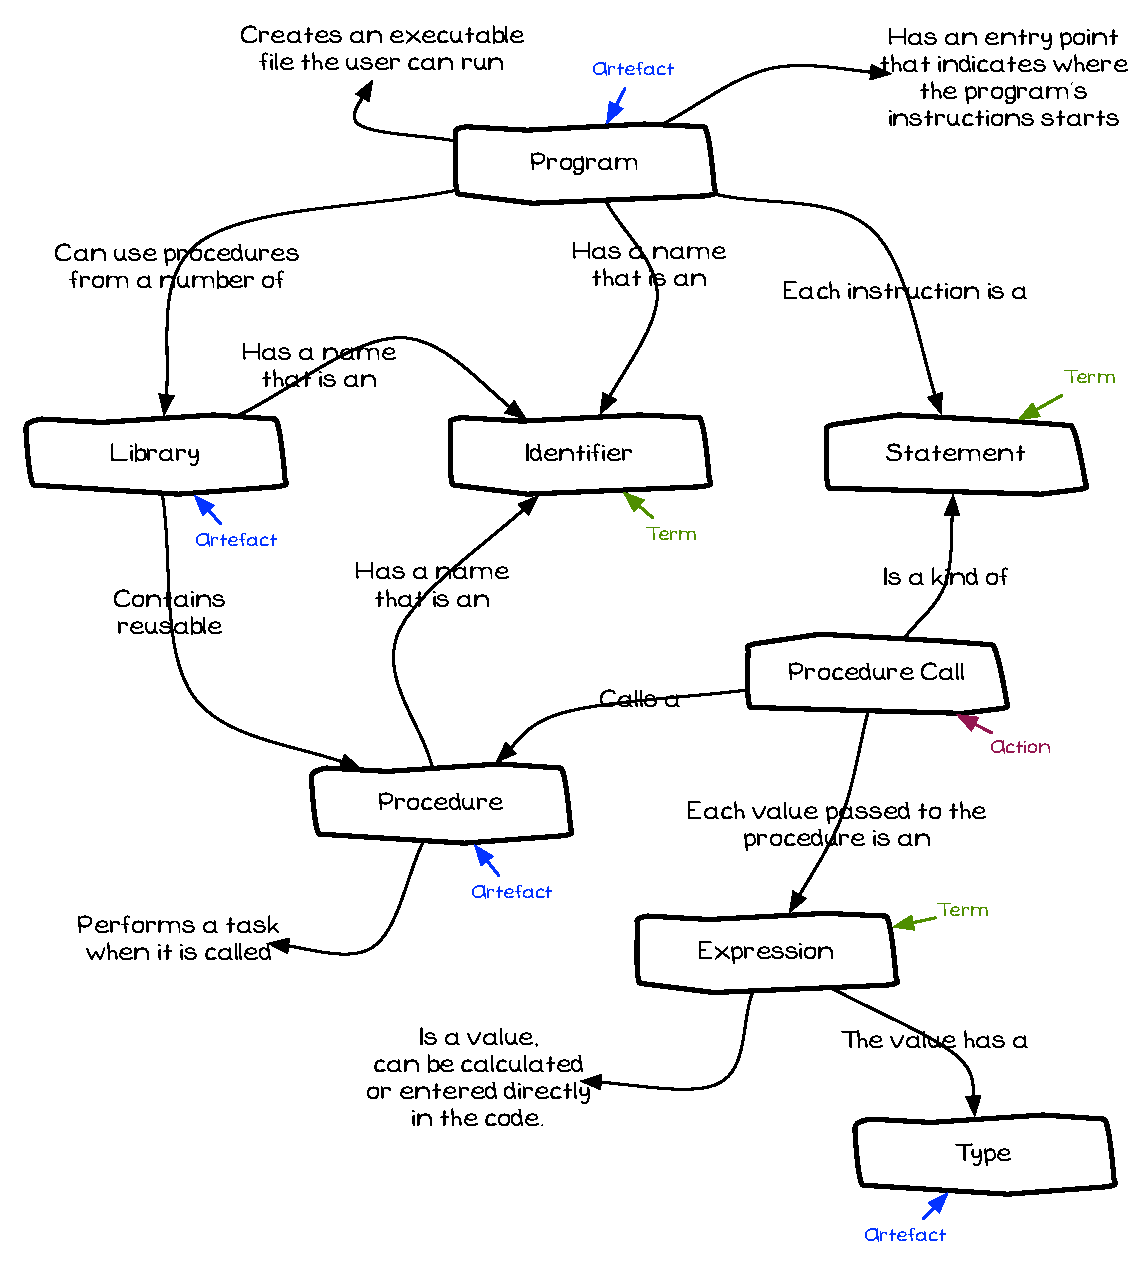
\includegraphics[width=\textwidth]{./topics/program-creation/diagrams/Summary} 
   \caption[Chapter Concepts]{Key Concepts introduced in this Chapter}
   \label{fig:program-creation-summary}
\end{figure}

\mynote{
\begin{itemize}
  \item \textbf{Artefacts} are things you can \emph{create} and \emph{use}.
  \item \textbf{Terms} are things you need to \emph{understand}.
  \item \textbf{Actions} are things you can \emph{command} the computer to perform.
\end{itemize}
}

% subsection summary (end)


% ======================
% = Using the Concepts =
% ======================

\clearpage
\section{Using these Concepts} % (fold)
\label{sec:using_these_concepts_program_creation}

Armed with the knowledge you have gained in the Section \ref{sec:program_creation_concepts} you can now start to design a small program.

\subsection{Designing Output Test} % (fold)
\label{sub:designing_hello_world}

Our first programming task is to extended the classic `Hello World' program to also output some data values, which we will call \textbf{Output Test}. This program will allow you to see all of the different concepts from this chapter in action. A description of the program is shown in Table \ref{tbl:program-creation-hello world description}, and a sample execution is shown in Figure \ref{fig:program-creation-helloworld2}.

\begin{table}[h]
\centering
\begin{tabular}{l|p{12cm}}
  \hline
  \multicolumn{2}{c}{\textbf{Program Description}} \\
  \hline
  \textbf{Name} & \emph{Output Test} \\
  \\
  \textbf{Description} & Displays the text \textbf{`Extended Hello World!'} on the Terminal, followed by \\
                       & \textbf{` 1 + 1 = '} and the result of the calculation 1 + 1, and then \\
                       & \textbf{` Area of a circle with radius 3 = '} and the result of calculating this value. \\
  \hline
\end{tabular}
\caption[Output Test Description]{Description of the \emph{Output Test} program.}
\label{tbl:program-creation-hello world description}
\end{table}

\begin{figure}[h]
   \centering
   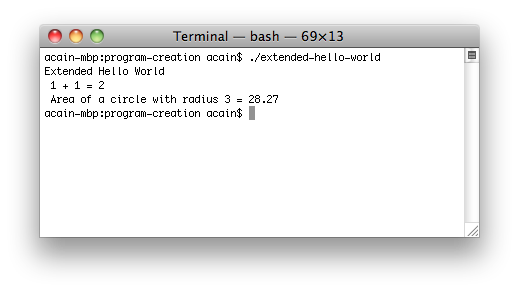
\includegraphics[width=\textwidth]{./topics/program-creation/images/HelloWorld} 
   \caption{Output Test run from the Terminal}
   \label{fig:program-creation-helloworld2}
\end{figure}

To design and implement this program we need to follow a number of steps:

\begin{enumerate}
  \item Understand the problem, and get some ideas on the tasks that need to be performed
  \item Choose the artefacts we will create and use
  \item Map these artefacts to code
  \item Compile and run the program
\end{enumerate}


% \begin{enumerate}
%   \item Determine the programming artefacts that you will need for the program; covered in section \ref{sub:choosing_artefacts_hello_world}. To do this you will need to:
%   \begin{itemize}
%     \item Decide which artefacts to \textbf{create}.
%     \item Select artefacts to \textbf{use} from the Libraries.
%   \end{itemize}
%   \item Determine the sequence of instructions you will need to give the computer for it to use these artefacts to produce the outcome you are looking for.
% \end{enumerate}


% subsection designing_hello_world (end)
\clearpage
\subsection{Understanding Output Test} % (fold)
\label{sub:understanding_output_test}

The first step in creating a program is to analyse the problem, and find related material that we can use to make sure we know what the computer needs to do. You need to understand what the program needs to do before you can start to design the solution.

For this program you need to understand how to calculate the answer of the equation 1 + 1, which is a trivial task, and also how to calculate the area of a circle given its radius. A quick search of the internet and you can find the equation is $PI \times r^2$. Using these equations you have the knowhow needed to calculate the values needed to be output.

% subsection understanding_output_test (end)
\subsection{Choosing Artefacts for Output Test} % (fold)
\label{sub:choosing_artefacts_hello_world}

Designing a program is all about making decisions around how to organise the program's instructions. This means \textbf{deciding} on which artefacts you will \textbf{create}, and which you will \textbf{use}. This chapter has introduced the concept of \textbf{creating} a \nameref{sub:program}, and \textbf{using} \nameref{sub:procedure}s. With these tools it is possible to design simple programs that will get the computer to perform actions by running Procedures in sequence.

The design of \emph{Output Test} requires:

\begin{itemize}
  \item The \textbf{creation} of a \nameref{sub:program}. This Program will contain the instructions to write the three messages to the Terminal.
  \item The \textbf{use} of a procedure to write to the Terminal. Programming languages provide a standard \nameref{sub:library} that, amongst other things, contains procedures to write data to the Terminal. This means you can call one of these procedures, passing it the data you want written to the Terminal, and let it take care of the details of how this is done.
\end{itemize}

\bigskip

The design for this program can be documented using a language neutral \textbf{pseudocode}. This isn't code, just a structured textural description of how the program is intended to work. It gives us a way of reasoning about the program we are creating that is independent of the language used to implement it. As this isn't really code it means we can write it without having to worry about the syntax of a specific programming language.

Listing \ref{lst:program-creation-hello-pseudo} shows the pseudocode for the \emph{Output Test} program. This represents the \textbf{Program} that needs to be created, and shows the three \textbf{procedure calls} that need to be made. 

\pseudocode{lst:program-creation-hello-pseudo}{Pseudocode for the Output Test program.}{./topics/program-creation/application/HelloWorld.txt}

\csection{In C the procedure to write data to the Terminal is called \texttt{printf}, see \nameref{sub:c_console_output}.}
\passection{Pascal has two procedures to write data to the Terminal, \texttt{Write} and \texttt{WriteLn}. }

% subsection choosing_artefacts (end)
\clearpage
\subsection{Writing the Code for Output Test} % (fold)
\label{sub:writing_the_code_for_output_test}

The pseudocode in Listing \ref{lst:program-creation-hello-pseudo} contains the instructions that will get the computer to perform the actions needed by the \emph{Output Test} program. These instructions are not in a form that can be used by the Computer, which can only use machine code. The next step is therefore to convert these ideas into source code that a compiler can then turn into machine code.

The following two sections, Section \ref{sec:program-creation-in-c} \nameref{sec:program-creation-in-c} and Section \ref{sec:program-creation-in-pas} \nameref{sec:program-creation-in-pas}, contain a description of the syntax needed to create programs in the C and Pascal programming languages. Each section outlines how to write the code so that it can be understood by the compiler. These are expressed as a number of related syntax rules. You will find the rules that you need to create a Program, the rules for calling a Procedure, and the related rules.

The rules themselves are expressed as \textbf{Syntax Diagrams}. An example diagram is shown in Figure \ref{synt:basic-rule}. This diagram shows the syntax related to two rules, \emph{first rule}, and \emph{second rule}, and shows the four main parts of all the Syntax Diagrams.

\begin{enumerate}
  \item Text found at the start of a line, not contained in a box, is the name of a rule. There are two rules in Figure \ref{synt:basic-rule}: \emph{first rule}, and \emph{second rule}.
  \item The arrows show the order in which the parts of the rule are applied. They start at the rule, and point in the direction you need to follow. Each box pointed to by the arrow represents either another rule to apply, or text that must be entered into the code at that point.
  \item The rectangular boxes on the line indicate points where other rules need to be applied. For example, the node  \tikz \node [nonterminal] {second rule}; within the \emph{first rule} indicates that you \textbf{must} apply the \emph{second rule} at this point.
  \item The boxes with rounded corners represent text that must be entered into the code. For example, the node \tikz \node [terminal] {write in the code}; within the \emph{first rule} indicates that you \textbf{must} write the text `\emph{write in the code}' at this point in your code.
\end{enumerate}

\examplesyntax{synt:basic-rule}{An example rule}{basic_rules}

In order to use these Syntax Diagrams, you must know what it is that you want to write in the code. The rules in Figure \ref{synt:basic-rule} indicate that you can write either a \emph{first rule} or a \emph{second rule}. If you want to write a \emph{first rule} you find that rule in the diagram, and then follow it's arrows. Reading the \emph{first rule} indicates that the \emph{second rule} must be applied first. 

The \emph{second rule} tells you that you must write the text `\emph{stuff to}'. The vertical bar at the end of the line indicates the end of the \emph{second rule}. This means at this stage the code is:

\begin{verb}
  stuff to 
\end{verb}

Having finished the \emph{second rule}, you can return back to finish the \emph{first rule}. This indicates that you need to write `\emph{write in the code}' in the code. This is the last part of the \emph{first rule}, and so the code needed to write a \emph{first rule} from the Syntax Diagram in Figure \ref{synt:basic-rule} is shown below.

\begin{verb}
  stuff to write in the code
\end{verb}

For a more realistic example have a look at the Syntax Diagram in Figure \ref{synt:example-identifier}\footnote{ 
The \tikz \node [meta-terminal] {...}; is used as shorthand to avoid having to list all of the characters between `A' to `Z'.}. This shows the rules you need to follow to code an \nameref{sub:identifier}\footnote{Most programming languages have the same rules for identifiers.} in either C or Pascal.

\examplesyntax{synt:example-identifier}{The Syntax Rules for an Identifier}{identifier}

There are three rules in Figure \ref{synt:example-identifier}, the \textbf{identifier} rule itself which uses the rules \textbf{letter} and \textbf{digit}. These rules show arrows that give you \emph{options}, and the ability to \emph{repeat} parts of the rules.

\begin{itemize}
  \item A \textbf{letter} is one alphabetic character: i.e. one of `A' to `Z' or `a' to `z'. This is an example of options in the syntax, where you follow \textbf{one} of the available arrows.
  \item A \textbf{digit} is a single number: i.e. a number between `0' and `9'.
  
  \item The \textbf{identifier} has a more complicated rule, with the following parts:
  \begin{enumerate}
    \item The first thing in an \nameref{sub:identifier} must be either a \emph{letter} or an underscore ( \_ ).
    \item Following this is an example of another kind of option. Here you have the ability to end the rule, allowing you to have identifiers that are a single character, or you can follow the downward arrow to include other letters, digits, and underscores.
    \item Following the downward arrow you have a new option where you can choose to have either a \emph{letter}, a \emph{digit}, or an underscore as the second character in your identifier.
    \item Continuing after this option you have another option where you can return back to repeat the previous step, allowing you to have identifiers with more than one or two characters.
  \end{enumerate}
\end{itemize}

\subsubsection{Using the Syntax Diagrams} % (fold)
\label{ssub:using_the_syntax_diagrams}

The Syntax Diagrams help you to map a Concept to the actual code that needs to be written in your source code. To use these diagrams you must first know what it is that you want to create or use, and then you can look up the related syntax. This is where the pseudocode code comes into play. It contains a description of the things that need to be created. 

Listing \ref{lst:program-creation-hello-pseudo3} shows the pseudocode for the Output Test program. This tells you what needs to be created; you need to create a \nameref{sub:program}. This means you need to find the syntax that tells you the rules of how a \emph{Program} is written in C or Pascal. 

\pseudocode{lst:program-creation-hello-pseudo3}{Pseudocode for the \emph{Output Test} program (repeated from Listing \ref{lst:program-creation-hello-pseudo})}{./topics/program-creation/application/HelloWorld.txt}

The pseudocode also indicates that you need to find the rules related to \nameref{sub:procedure call}s. For this Program you need to code three procedure calls within the program's instructions. The language's syntax will tell you how you code these instructions, the Syntax for the program will show you where these instructions are written.

% subsubsection using_the_syntax_diagrams (end)

\subsubsection{How the Syntax is Presented} % (fold)
\label{ssub:how_the_syntax_is_presented}

The C and Pascal Syntax needed to create a program are shown in Section \ref{sec:program-creation-in-c} \nameref{sec:program-creation-in-c} and Section \ref{sec:program-creation-in-pas} \nameref{sec:program-creation-in-pas}. Each part of the Syntax is presented on its own page that shows the Syntax Diagram followed by an example and some notes. The best way to approach this is to do the following:

\begin{enumerate}
  \item Find the page with the Syntax rule you are interested in knowing about.
  \item Have a quick look at the Syntax Diagram and the rules it contains. Read each rule, and get a basic feel for how it is going to come together for your program.
  \item Read the example to see one way of using the Rule. The Syntax Diagram can be used to create any number of variations of the rule, the example gives you at least one way these rules can be coded.
  \item Return to the diagram and make sure you can match each part of the example back to the rule that created it.
  \item Now look up any related rules that are not explained on this rule's page. For example, a \nameref{sub:program} will use the \nameref{sub:statement} rule to code its instructions. The actual rule for a Statement will have its own page. When you read the rules for a Program you will need to also find the page with the rules for a Statement so that you know how to code these within the program.
\end{enumerate}

As you follow this process it is also a good idea to try to use these rules in your own program. Have your code editor open, and see if you can follow the rules or mimic the examples to start building your own program's code. You can also try typing in some of the examples to see how they work.

% subsubsection how_the_syntax_is_presented (end)

% subsection writing_the_code_for_output_test (end)

\subsection{Compiling and Running Output Test} % (fold)
\label{sub:compiling_and_running_output_test}

The previous sections have shown the pseudocode for the \emph{Output Test} program. These steps can be coded using either C or Pascal into a source code file. In order to actually use these instructions you will first need to \textbf{compile} the source code file. This will produce an executable file that you can run.

We are going to start using a \textbf{command line compiler}. You will run this compiler within a text based environment, the \textbf{Terminal}. 

\begin{itemize}
  \item On Ubuntu \textbf{Linux} you can find the Terminal in the \textbf{Accessories} folder within \textbf{Applications}. See Figure \ref{fig:program-creation-ubuntu-terminal}.
  \item On \textbf{MacOS} you can find the Terminal in the \textbf{Utilities} folder within \textbf{Applications}. See Figure \ref{fig:program-creation-macos-terminal}.
  \item On \textbf{Windows} you will need to download and install \emph{MinGW}, making sure to select the \emph{MinSYS} option during the install process. The \emph{MinGW Shell} is then the equivalent of Terminal on the other operating systems. You will find this in \textbf{Program Files}, \textbf{MinGW}. See Figure \ref{fig:program-creation-mingw-shell}.
\end{itemize}

\begin{figure}[p]
   \centering
   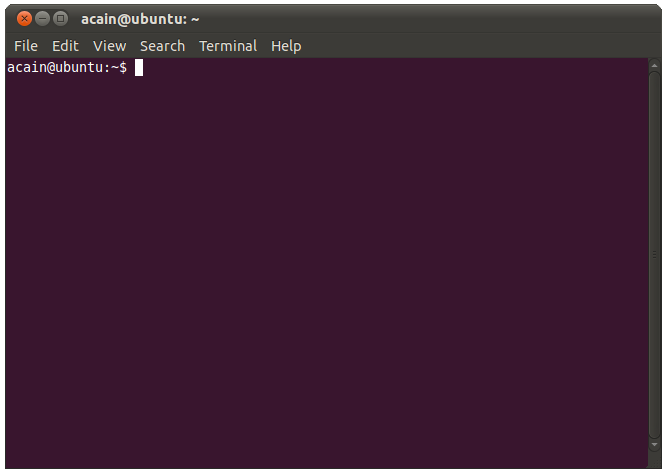
\includegraphics[width=0.6\textwidth]{./topics/program-creation/images/UbuntuTerminal} 
   \caption{Terminal on Ubuntu Linux}
   \label{fig:program-creation-ubuntu-terminal}
\end{figure}

\begin{figure}[p]
   \centering
   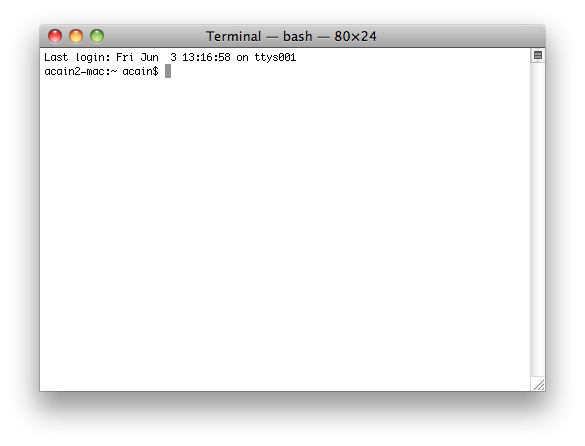
\includegraphics[width=0.6\textwidth]{./topics/program-creation/images/MacOSTerminal} 
   \caption{Terminal on MacOS}
   \label{fig:program-creation-macos-terminal}
\end{figure}

\begin{figure}[p]
   \centering
   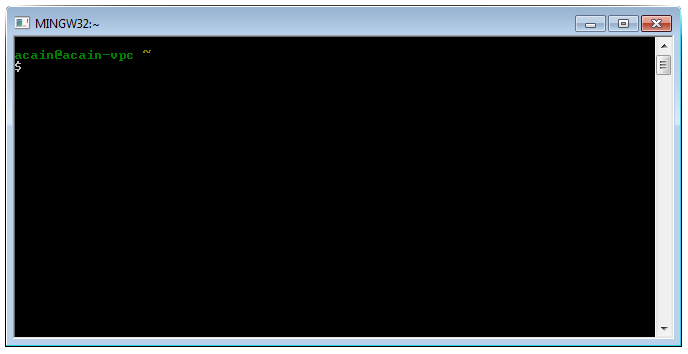
\includegraphics[width=0.6\textwidth]{./topics/program-creation/images/MinGWShell} 
   \caption{MinGW Shell, the Terminal for Windows}
   \label{fig:program-creation-mingw-shell}
\end{figure}

Once you are in the Terminal you have the ability to run a number of text based commands. These commands instruct the computer to perform actions for you.

\begin{itemize}
  \item \textbf{pwd} stands for \emph{Present Working Directory}, and shows you where you are in the file system.
  \item \textbf{ls} stands for \emph{List} and it prints out a list of the files that are in the current directory.
  \item \textbf{cd} stands for \emph{Change Directory} and it moves you to another directory. 
\end{itemize}

To compile your program you need to do the following:

\begin{enumerate}
  \item Change into the directory where your code is located using the \textbf{cd} command. For example, if your code is in a \emph{Code} folder in your \emph{Documents} folder you would use:
  \begin{itemize}
    \item \textbf{Linux}: \texttt{cd /home/username/Documents/Code}
    \item \textbf{MacOS}: \texttt{cd /Users/username/Documents/Code}
    \item \textbf{Windows}: \texttt{cd /c/Users/username/Documents/Code}\footnote{This example moves you into the \texttt{c:{\textbackslash}Users{\textbackslash}username{\textbackslash}Documents{\textbackslash}Code} folder. You need to use the /c/ to refer to the C drive. }
  \end{itemize} 
  \item Run the compiler, passing in the name of the file you want to compile. See the language specific notes below
  \item Execute the program using \texttt{./OutputTest}
\end{enumerate}

\csection{
The C compiler is called \textbf{gcc}. To compile your \emph{Output Test} program you will need to run the following: \bashcode{}{}{code/c/program-creation/compile-output-test.sh}
}

\passection{
The Pascal compiler is called \textbf{fpc}. To compile your \emph{Output Test} program you will need to run the following: \bashcode{}{}{code/pascal/program-creation/compile-output-test.sh}
}

\clearpage
Figure \ref{fig:program-creation-complete-linux-version} shows an example of the instructions needed to compile and run the C version of the \emph{Output Test} program on Linux. Figure \ref{fig:program-creation-complete-linux-version-1} shows an example of the instructions needed to compile and run the Pascal version of the \emph{Output Test} program on Linux.

\begin{figure}[h]
   \centering
   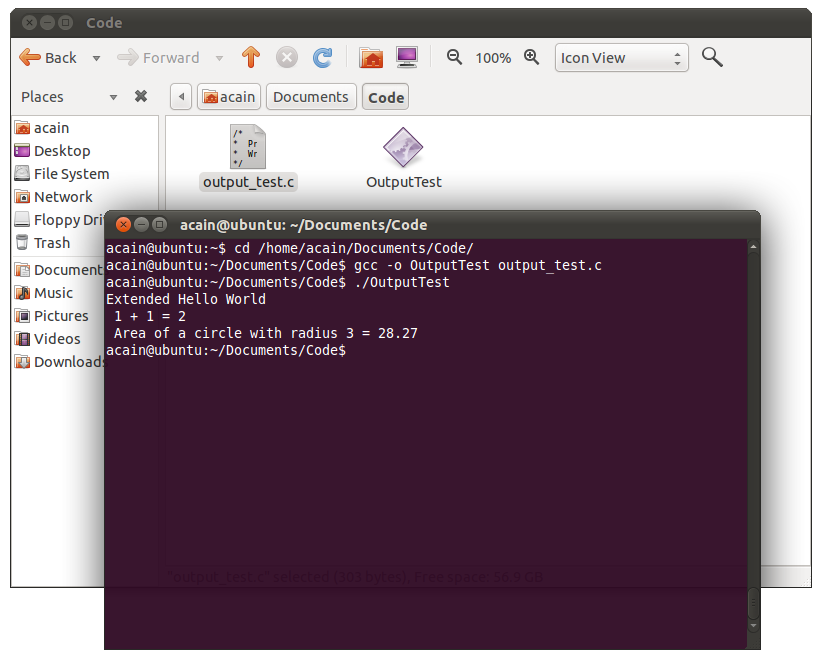
\includegraphics[width=0.62\textwidth]{./topics/program-creation/images/LinuxCompleteExample1} 
   \caption{Example of compiling and running a C version of Output Test on Linux}
   \label{fig:program-creation-complete-linux-version}
\end{figure}

\begin{figure}[h]
   \centering
   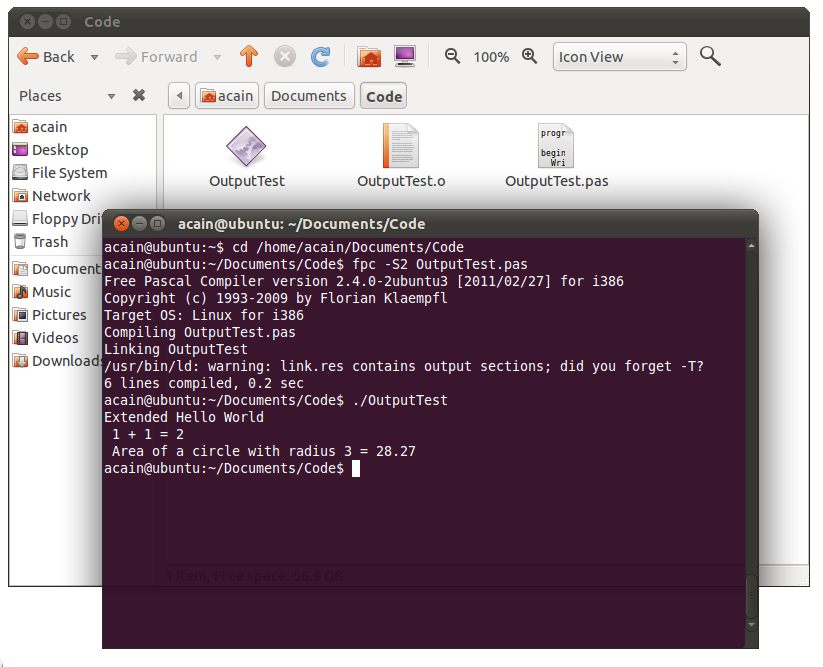
\includegraphics[width=0.62\textwidth]{./topics/program-creation/images/LinuxCompleteExample} 
   \caption{Example of compiling and running a Pascal version of Output Test on Linux}
   \label{fig:program-creation-complete-linux-version-1}
\end{figure}

\clearpage
Figure \ref{fig:program-creation-complete-macos-version} shows an example of the instructions needed to compile and run the C version of the \emph{Output Test} program on MacOS. Figure \ref{fig:program-creation-complete-macos-version-1} shows an example of the instructions needed to compile and run the Pascal version of the \emph{Output Test} program on MacOS.

\begin{figure}[h]
   \centering
   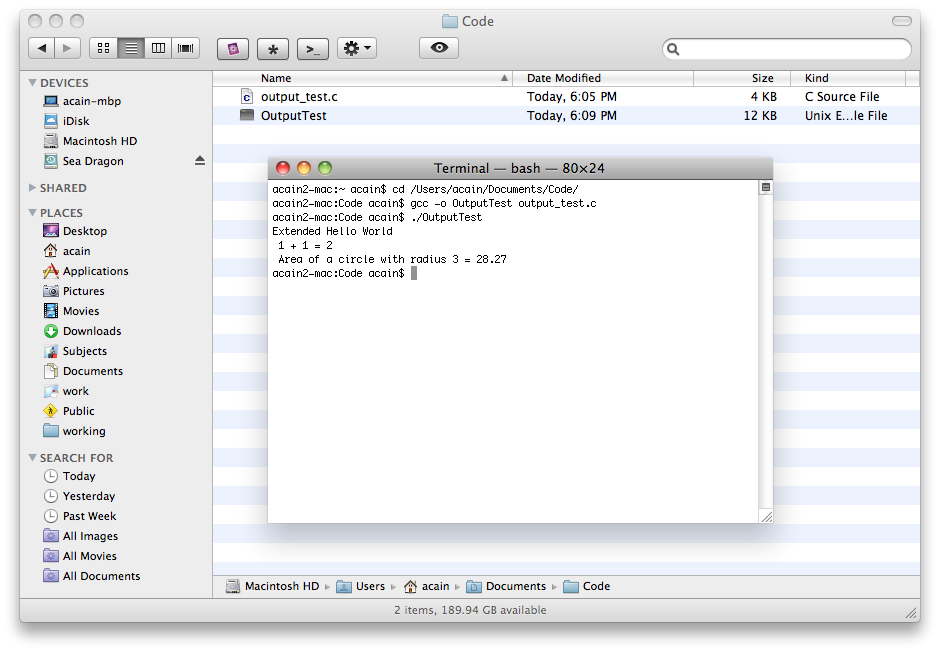
\includegraphics[width=0.73\textwidth]{./topics/program-creation/images/MacOSCompleteExample1} 
   \caption{Example of compiling and running a C version of Output Test on MacOS}
   \label{fig:program-creation-complete-macos-version}
\end{figure}

\begin{figure}[h]
   \centering
   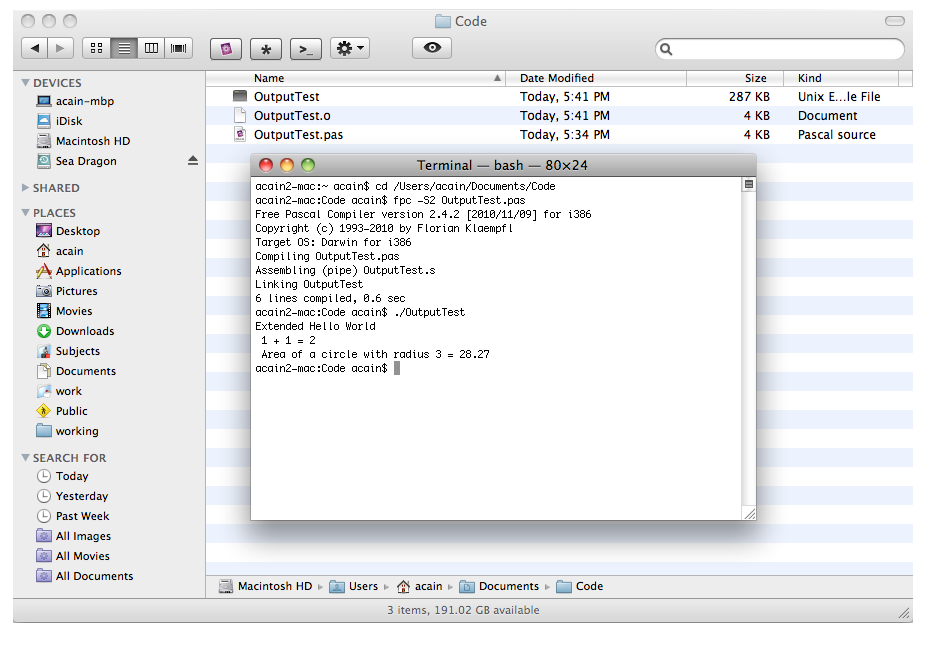
\includegraphics[width=0.73\textwidth]{./topics/program-creation/images/MacOSCompleteExample} 
   \caption{Example of compiling and running a Pascal version of Output Test on MacOS}
   \label{fig:program-creation-complete-macos-version-1}
\end{figure}

\clearpage
Figure \ref{fig:program-creation-complete-windows-version} shows an example of the instructions needed to compile and run the C version of the \emph{Output Test} program on MacOS. Figure \ref{fig:program-creation-complete-windows-version-1} shows an example of the instructions needed to compile and run the Pascal version of the \emph{Output Test} program on MacOS.

\begin{figure}[h]
   \centering
   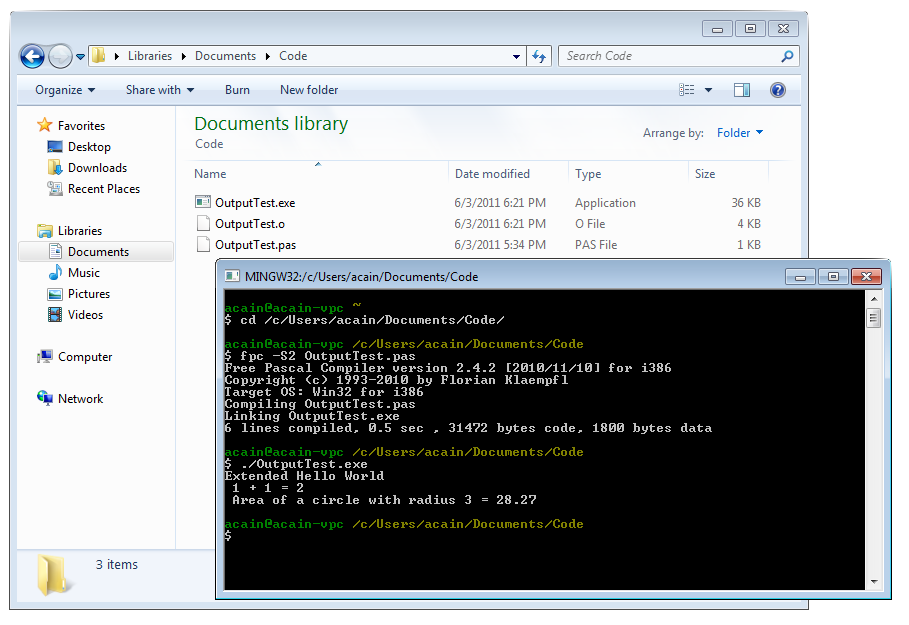
\includegraphics[width=0.73\textwidth]{./topics/program-creation/images/WindowsCompleteExample} 
   \caption{Example of compiling and running a C version of Output Test on Windows}
   \label{fig:program-creation-complete-windows-version}
\end{figure}

\begin{figure}[h]
   \centering
   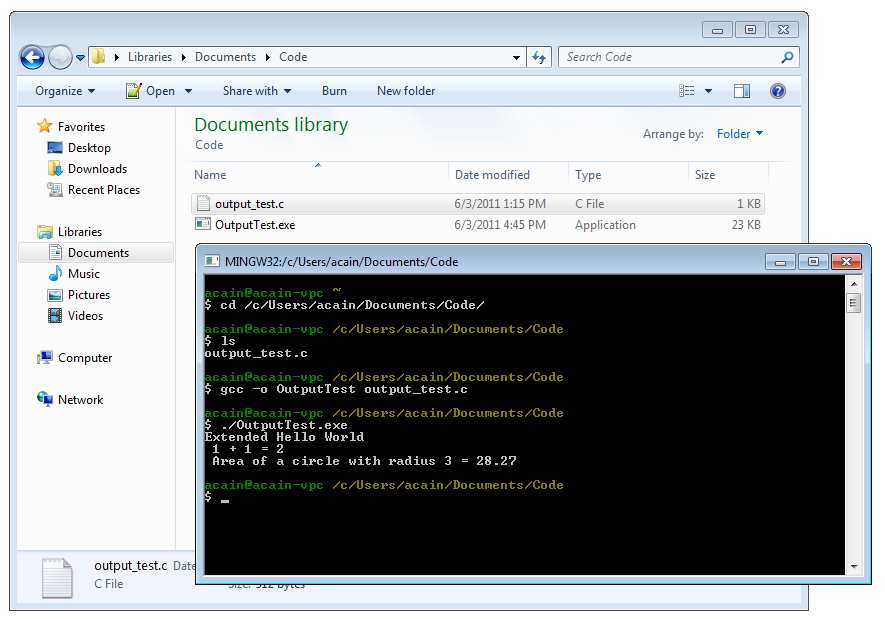
\includegraphics[width=0.73\textwidth]{./topics/program-creation/images/WindowsCompleteExample1} 
   \caption{Example of compiling and running a C version of Output Test on Windows}
   \label{fig:program-creation-complete-windows-version-1}
\end{figure}

% subsection compiling_and_running_output_test (end)
\clearpage
\subsubsection{Compiler Errors} % (fold)
\label{ssub:compiler_errors}

The compiler is a very sensitive piece of software. It requires that you follow the language's syntax precisely. One small mistake, and the compiler will fail to compile your program and end with an error message. This is further complicated by the fact that in many cases the compiler's error messages can appear cryptic.

Here are some handy hints related to dealing with compiler errors.

\begin{enumerate}
  \item \textbf{Know that errors are inevitable}. You will get compiler errors. As you gain more experience you will get fewer errors, but it will always be a rare event that everything is exactly as it should be the first time.
  \item \textbf{Start with the first error message, and do not move on until its fixed}. The compiler will read your code from the top down. So the first error it outputs will be the first in the file. The problem is that the compiler will try to continue on, despite the error. This can mean that other errors further on it the output were actually caused by the compiler being \emph{confused} due to the first error. By fixing the first error you may also fix subsequent errors, as you gain experience you will learn to work out which errors are genuine, and which were caused by previous errors.
  \item \textbf{Deal with one error at a time}. Its easy to feel overwhelmed when you see a huge list of errors, but do not be scared off. Start at the first error, and solve them one by one. Compile after fixing each problem to see if the others are real, or if they were a result of the previous error.
  \item \textbf{Do not add more code until the errors are fixed}. Compile your program frequently. Add small pieces of functionality, and then fix any syntax errors before adding the next piece of functionality. Coding in this way makes sure that you should not get too many errors, and reduces the code you have to search in order to fix the problem.
  \item \textbf{Read the error message carefully}. The message will try to tell you what has gone wrong, and once you understand what the messages are trying to say you will be able find and fix the issues quickly.
  \item  \textbf{Work out what the error messages mean}. Understanding the error messages will mean that you will know what to look for, and will help you avoid these errors in the future. If your not sure what an error message means ask others developers or search for the message on the internet.
  \item \textbf{Find the line and character number of the error}. One important detail in the error message will be the line number of the error. This gives you a starting point to help you locate the problem. Its important to note that this is where the compiler got to when it noticed the error. This \emph{does not} guarantee that this is where the error actually is, but it is a good place to start looking. In some cases this will be the location of the error, in others you may need to look back one or more lines to find the actual source of the problem.
  \item \textbf{Watch for typos}. It is easy to mistype an identifier. When this happens the compiler will not know what to do. Make sure you check for these tiny typos when you get errors related to the compiler not being able to find an identifier.
  \item \textbf{When you get stuck ask for help}. Compiler errors are likely to be something small, but something these small things are hard to find. If you get stuck ask for help. Having access to other more experienced developers will be a valuable resource as you learn to program. Learning to program can be tough at times, and having someone who can help you will make all the difference.
\end{enumerate}


% subsubsection compiler_errors (end)



% section using_these_concepts (end)


% =============
% = C Section =
% =============
\clearpage
\def\pageLang{c}
\section{Program Creation in C}
\label{sec:program-creation-in-c}

% Overview of concepts in C
Section \vref{sec:using_these_concepts_program_creation} of this chapter introduced an `Output Test' program, and its design. The pseudocode from this section is shown in Listing \ref{lst:program-creation-hello-pseudo 1}. In this Section you will see the rules for translating this program's design into the C code shown in Listing \ref{lst:program-c-output_test}.

\pseudocode{lst:program-creation-hello-pseudo 1}{Pseudocode for Hello World program (from Listing \ref{lst:program-creation-hello-pseudo}).}{./topics/program-creation/application/HelloWorld.txt}

\csection{\ccode{lst:program-c-output_test}{Output Test in C}{code/c/program-creation/output_test.c}}

\mynote {
\begin{itemize}
  \item Save the C code in a file named \texttt{output\_test.c}.
  \item Compile this using \bashsnipet{gcc -o:OutputTest output_test.c}.
  \item Run using \bashsnipet{./OutputTest}.
  \item The code at the start is a Comment describing what is in the file, see \nameref{sub:c_comments}.
  \item The code \csnipet{#include <stdio.h>}, is part of the \nameref{sub:program_in_c}. It is a \emph{header include}, and gives access to the code in the \emph{Standard IO} Library.
  \item \csnipet{int main() { ... }} is part of the \nameref{sub:program_in_c}, it marks the entry point and contains the instructions that are executed when the program runs.
  \item The \texttt{main} function contains three \nameref{sub:program-creation-c_procedure_call}s. Each is a call to the \texttt{printf}. \nameref{sub:procedure}, which is used to output text to the console. See \nameref{sub:c_console_output}.
  \item Each of the procedure calls contains one or two \nameref{sub:expression}s that pass values to the \texttt{printf} procedure, which will output these to the Terminal.
  \item This code uses \texttt{c-strings}, \texttt{int}, and \texttt{float} types, see \nameref{sub:program-creation-c_types}.
\end{itemize}
}

% Each part of the syntax
% \clearpage
% \subsection{C++ Program} % (fold)
% \label{sub:program_in_c}

% The C++ programming language does not have an explicit Program artefact for you to create. Rather, in C++ a program is implied by the existence of a special function called `\texttt{main}' somewhere in your source code. Figure \ref{csynt:program-creation-program} shows the structure of the syntax you can use to create a program using the C++ language.

% \csyntax{csynt:program-creation-program}{a Program}{program-creation/program}

% The code in Listing \ref{lst:program-creation-c-hello-world} shows an example C++ Program. You should be able to match this up with the syntax defined in Figure \ref{csynt:program-creation-program}. Notice at the start of the code the syntax indicates we can have an optional \emph{header include}, this matches up with the first line in the code where it \emph{includes} the `splashkit.h' header file. Declaration of the \texttt{main} function follows the inclusion of the header file, and it contains the instructions that are executed when the program runs.

% \csection{\ccode{lst:program-creation-c-hello-world}{C++ Hello World}{code/c/program-creation/hello-world.c}}

% \mynote{
%   \begin{itemize}
%     \item When a C++ \nameref{sub:program} runs, it start running the instructions from the first \nameref{sub:statement} within the \texttt{main} function (line 5).
%     \item A \nameref{sub:function} is a kind of \nameref{sub:procedure}, and their details will be covered later (see \sref{sub:function}).
%     \item The `\texttt{return 0}' code is a \nameref{sub:statement} that ends the \texttt{main} function (and the program). The \nameref{sub:return_statement} is covered later in \sref{sub:return_statement}.
%     \item With the \emph{header include} syntax you use \csnipet{#include <...>} to include standard libraries, and \csnipet{#include "..."} to include other external libraries.
%     \item Header files contain a summary of the features available within a library. By including the header file you gain access to these features.
%   \end{itemize}
% }

% % subsection program_in_c (end)
\clearpage
\subsection{C Statement} % (fold)
\label{sub:program-creation-c_statement}

In a \nameref{sec:program-creation-statement} you are commanding the computer to perform an action. There are only a small number of statements you can choose from. At this stage the only statement is the \nameref{sub:procedure call}, known as the \emph{procedure statement} in C. This is shown in Figure \ref{csynt:program-creation-statement}, where we can see that at this stage all Statements are calls to \nameref{sub:procedure}s.

\csyntax{csynt:program-creation-statement}{Statement Syntax}{program-creation/statement}

\csection{\ccode{lst:program-creation-c-knights}{C Knights}{code/c/program-creation/knights.c}}

\mynote{
\begin{itemize}
  \item The code in Listing \ref{lst:program-creation-c-knights} contains a \nameref{sub:program_in_c}.
  \item This Program contains five procedure calls, see \nameref{sub:program-creation-c_procedure_call}.
  \item Each procedure call runs the \texttt{printf} procedure to output text to the console. See the section on \nameref{sub:c_console_output}.
\end{itemize}
}


% subsection c_statement (end)
\clearpage
\subsection{C Procedure Call} % (fold)
\label{sub:program-creation-c_procedure_call}

A Procedure Call allows you to run the code in a Procedure, getting its instructions to run before control returns back to this point in the Program.

\csyntax{csynt:program-creation-procedure-call}{Procedure Call Syntax}{program-creation/procedure-call}

\csection{\ccode{lst:program-creation-c-count-back}{C Count Back}{code/c/program-creation/count-back.c}}

\mynote{
\begin{itemize}
  \item A Procedure Call is an \textbf{action}, it commands the computer to run the code in a Procedure.
  \item The Procedure Call starts with the Procedure's \nameref{sec:program-creation-identifier}, this indicates the procedure to be called.
  \item Following the Identifier is a list of values within parenthesis,  these are the values (coded as \nameref{sub:expression}s) that are passed to the procedure for it to use.
  \item Remember that C is case sensitive so using \texttt{Printf} instead of \texttt{printf} will not work.
  \item The code in Listing \ref{lst:program-creation-c-count-back} contains a \nameref{sub:program_in_c}.
  \item This Program contains four procedure calls.
  \item Each procedure call runs the \texttt{printf} procedure to output text to the console. See the section on \nameref{sub:c_console_output}.
  
\end{itemize}
}


% subsection c_procedure_call (end)
\clearpage
\subsection{C Identifier} % (fold)
\label{sub:c_identifier}

The C \nameref{sec:program-creation-identifier} syntax is shown in Figure \ref{csynt:program-creation-identifier}. In C, as in most languages, the identifier must start with an underscore (\_) or a letter, in other words your identifiers cannot start with a number or contain other symbols. This is because the compiler needs a way of distinguishing identifiers from numbers entered in the code as Literals.

\csyntax{csynt:program-creation-identifier}{an Identifier}{program-creation/identifier}

\begin{table}[h]
  \centering
  \begin{tabular}{|ccccc||cc|}
    \hline
    \multicolumn{5}{|c||}{\textbf{Keywords}} & \multicolumn{2}{c|}{\textbf{Example Identifiers}} \\
    \hline
    \texttt{auto}     &   \texttt{break}    & \texttt{case}     &   \texttt{char}     &   \texttt{const}   & printf & scanf  \\         
    \texttt{continue} &   \texttt{default}  &  \texttt{do}      &   \texttt{double}   &   \texttt{else}    & bitmap & sound\_effect  \\
    \texttt{enum}     &   \texttt{extern}   & \texttt{float}    &   \texttt{for}      &   \texttt{goto}    & name & draw\_bitmap  \\
    \texttt{if}       &   \texttt{int}      &   \texttt{long}   &   \texttt{register} &   \texttt{return}  & age & my\_alien \\         
    \texttt{short}    &   \texttt{signed}   & \texttt{sizeof}   &   \texttt{static}   &   \texttt{struct}  & height & test  \\          
    \texttt{switch}   & \texttt{typedef}  &   \texttt{union}    &   \texttt{unsigned} &   \texttt{void}    & alien & name3 \\
    \texttt{volatile} &   \texttt{while}    &  & &                                                         & \_23  & i \\
    \hline
  \end{tabular}
  \caption{C Keywords and example Identifiers}
  \label{tbl:program-creation-c identifiers and keywords}
\end{table}












\mynote{
\begin{itemize}
  \item Table \ref{tbl:program-creation-c identifiers and keywords} contains a list of the keywords in C, and some example identifiers.
  \item Each item in Table \ref{tbl:program-creation-c identifiers and keywords} is a valid identifier.
  \item A letter is any alphabetic character (\emph{a} to \emph{z} and \emph{A} to \emph{Z}).
  \item A digit is a single number (\emph{0} to \emph{9}).
  \item A \textbf{keyword} is a kind of identifier that has special meaning to the language. Usually used to identify a kind of action, or a kind of artefact.
  \item Notice in the syntax definition that Identifiers cannot contain spaces, or special characters other than underscores (\_).
\end{itemize}
}

% subsection c_identifier (end)
\clearpage
\subsection{C Expression} % (fold)
\label{sub:program-creation-c_expression}

An \nameref{sub:expression} in C is a mathematical calculation or a Literal value. Each expression will have a \nameref{sub:type}, and can contain a number of mathematic operators. Table \ref{tbl:program-creation-c operators and expresions} lists the operators that you can include in your expressions, listed in order of precedence\footnote{The expressions follow the standard mathematic order of precedence (BODMAS).}. The operators you can use depend on the kind of data that you are using within the expression.

\begin{table}[h]
  \centering
  \begin{tabular}{|c|l|l|}
    \hline
    \textbf{Operator} & \textbf{Description} & \textbf{Example} \\
    \hline
    \texttt{ () }     &   Parenthesis                 & \texttt{(1 + 1) * 2}  \\
    \texttt{* /}      &   Multiplication and Division & \texttt{1 / 2 * 5}    \\
    \texttt{+ -}      &   Addition and subtraction    & \texttt{10 + 3 - 4}   \\
    \hline
  \end{tabular}
  \caption{C Operators and Example Expressions}
  \label{tbl:program-creation-c operators and expresions}
\end{table}

\begin{table}[h]
  \begin{minipage}{\textwidth}
  \centering
  \begin{tabular}{|c|c|l|}
    \hline
    \textbf{Example Expression} & \textbf{Value} & \textbf{Type} \\
    \hline
    \texttt{ 73 }     &   73                 & \texttt{int}  \\
    \texttt{ 2.1 }      & 2.1   & \texttt{float}    \\
    \texttt{ "Hello World" }      &   "Hello World"    & \texttt{char*}   \\
    \texttt{ "Fred" }      &   "Fred"    & \texttt{char*}   \\
    \texttt{ 3 * 2 } & 6 & \texttt{int} \\
    \texttt{ 1 + 3 * 2 }  & 7 & \texttt{int} \\
    \texttt{ (1 + 3) * 2} & 8 & \texttt{int} \\
    \texttt{ 7 - 3 + 1 }  & 5 & \texttt{int} \\
    \texttt{ 3 / 2 } & 1\footnote{C does integer division for int values, rounding the value off.} & \texttt{int} \\
    \texttt{ 3.0 / 2.0} & 1.5 & \texttt{float} \\
    \texttt{ 3 / 2.0 } & 1.5\footnote{If either or both value are real numbers the result is also a real number.} & \texttt{float} \\
    \texttt{ 1 + (3 / 2.0) + 6 * 2 - 8} & 6.5 & \texttt{float} \\
    \hline
  \end{tabular}
\end{minipage}
  \caption{C Operators and Example Expressions}
  \label{tbl:program-creation-c example expresions}
\end{table}


\mynote{
\begin{itemize}
  \item Table \ref{tbl:program-creation-c example expresions} shows some example expressions, their values, and types
  \item Expressions can be Literal values, entered in the code.
  \item Expression can contain mathematical calculations using standard addition, subtraction, multiplication, division, and grouping.
\end{itemize}
}


% subsection c_expression (end)
\clearpage
\subsection{C Literal} % (fold)
\label{sub:program-creation-c_literal}

A Literal is either a number or text value entered directly into the code. Figure \ref{csynt:program-creation-literal} shows the syntax for the different Literal values you can enter into your C code.

\csyntax{csynt:program-creation-literal}{Literals}{program-creation/literal}

\mynote{
\begin{itemize}
  \item Within a string the {\textbackslash} is used to indicate the next character has a special meaning. The following list includes the most useful escape characters:
  \begin{itemize}
    \item \texttt{{\textbackslash}n} creates a new line
    \item \texttt{{\textbackslash}"} creates a double quote
    \item \texttt{{\textbackslash}\%} creates a \% character
    \item \texttt{{\textbackslash}{\textbackslash}} creates a {\textbackslash}
  \end{itemize}
  % \item `0..9' means the digits 0, 1, 2, etc. up to 9.
  \item `\emph{any character except ", {\textbackslash}, \%, or new line}' allows you to include any character, with those that can not be includes directly being able to be included using the escape sequence (e.g. {\textbackslash}n for new line).
\end{itemize}
}

% subsection c_literal (end)
\clearpage
\subsection{C Types} % (fold)
\label{sub:program-creation-c_types}

\nameref{sub:type}s are used to define how data is interpreted and the operations that can be performed on the data. Table \ref{tbl:program-creation-c-types} shows the three basic types of data, the associated C type, size in memory, and other related information. Table \ref{tbl:program-creation-c operators by type} shows the operators that are permitted for each Type.

\begin{table}[h] 
\begin{minipage}{\textwidth}
\centering
\begin{tabular}{|l|c|c|c|}
\hline
\multicolumn{4}{|c|}{\textbf{Whole Number Types}} \\
\hline
\emph{Name} & \emph{Size} & \multicolumn{2}{|c|}{\emph{Range (lowest .. highest)}} \\
\hline
\texttt{short} & 2 bytes/16 bits & \multicolumn{2}{|c|}{-32,767 .. 32,767} \\
\texttt{int} & 4 bytes/32 bits & \multicolumn{2}{|c|}{-2147483648 .. 2147483647} \\
\texttt{long long}    & 8 bytes/64 bits & \multicolumn{2}{|c|}{-9,223,372,036,854,775,807 ..} \\
  & & \multicolumn{2}{|c|}{9,223,372,036,854,775,807} \\
\hline
\multicolumn{4}{c}{} \\
\hline
\multicolumn{4}{|c|}{\textbf{Real Number Types}} \\
\hline
\emph{Name} & \emph{Size} & \emph{Range (lowest .. highest)} & \emph{Significant Digits} \\
\hline
\texttt{float} & 4 bytes/32 bits & 1.0e-38 .. 1.0e38 & 6 \\
\texttt{double} & 8 bytes/64 bits & 2.0e-308 .. 2.0e308 & 10 \\
\hline
\multicolumn{4}{c}{} \\
\hline
\multicolumn{4}{|c|}{\textbf{Text Types}} \\
\hline
\emph{Name} & \emph{Size} & \multicolumn{2}{|c|}{\emph{Known As}} \\
\hline
\texttt{char}  & 1 byte/8 bits & \multicolumn{2}{|c|}{} \\
\hline
\texttt{char*} & various\footnote{1 byte per character + 1 byte overhead} &  \multicolumn{2}{|c|}{c-string} \\
\hline
\end{tabular}
\caption{C Data Types}\label{tbl:program-creation-c-types}
\end{minipage}
\end{table}

\begin{table}[h]
  \centering
  \begin{tabular}{|c|c|l|}
    \hline
    \textbf{Type} & \textbf{Operations Permitted} & \textbf{Notes}\\
    \hline
    Whole Numbers     &   \texttt{( ) + - / *} & Division rounds down if all\\
                                    &                        & values are whole numbers.\\
    Real Numbers   &   \texttt{( ) + - / *} &    \\
       & & \\
    Text           &   \texttt{( ) }          & You cannot perform mathematical\\
    & & operations on text.\\
    \hline
  \end{tabular}
  \caption{C Permitted Operators by Type}
  \label{tbl:program-creation-c operators by type}
\end{table}

\csyntax{csynt:program-creation-typed-literal}{Typed Literals}{program-creation/typed-literal}

\mynote{
\begin{itemize}
  \item The \texttt{int} type is the typical whole number type.
  \item The \texttt{double} type is the typical real number type.
  \item C has limited support for text data. In most languages, text is represented using a \texttt{String} type. The C text type is named \texttt{c-string} to indicate this limited support. C includes a \nameref{sub:library} to add operations to manipulate \texttt{c-string} values.
  \item For example values see Table \vref{tbl:program-creation-c example expresions}.
\end{itemize}
}
% subsection c_types (end)
\clearpage
\subsection{C Terminal Output} % (fold)
\label{sub:c_console_output}

C comes with a range of \nameref{sub:library}s that provide reusable programming artefacts, including reusable \nameref{sub:procedure}s. The Standard Library includes a number of different components, one of which is \texttt{stdio.h}. The \texttt{stdio.h} refers to the Standard Input/Output library. This header file gives you access to artefacts you can use to perform input and output, including code to write output to the Terminal. The \texttt{printf} procedure is used to write data to the Terminal.

\begin{table}[h]
  \centering
  \begin{tabular}{|c|p{9cm}|}
    \hline
    \multicolumn{2}{|c|}{\textbf{Procedure Prototype}} \\
    \hline
    \multicolumn{2}{|c|}{} \\
    \multicolumn{2}{|c|}{\texttt{printf(char *format, \ldots )}} \\
    \multicolumn{2}{|c|}{} \\
    \hline
    \textbf{Parameter} & \textbf{Description} \\
    \hline
    \texttt{ format } & The text that is to be written to the Terminal. This text may contain format tags to include other values. See Figure \ref{csynt:program-creation-format-string} for the syntax of the format tag. \\
    & \\
    \texttt{\ldots}   & Optional values, must have at least as many values as format tags. \\
    \hline
  \end{tabular}
  \caption{Parameters that must be passed to \texttt{printf}}
  \label{tbl:program-creation-c printf parameters}
\end{table}

The syntax for the \texttt{Format Tag} is shown in Figure \ref{csynt:program-creation-format-string}, with the details for the values that can be placed in the \emph{flag}, \emph{width}, \emph{precision}, and \emph{specifier} section being shown in Table \vref{tbl:program-creation-c printf specifier}. A number of examples are shown in Table \ref{tbl:program-creation-c printf specifier}, as well as in Listing \ref{lst:program-creation-c-printf}.

\csyntax{csynt:program-creation-format-string}{Format Tag}{program-creation/format-string}

\csection{\ccode{lst:program-creation-c-printf}{C \texttt{printf} Examples}{code/c/program-creation/sample-printf.c}}

\begin{table}[htbp]
  \begin{minipage}{\textwidth}
  \centering
  
  \begin{tabular}{|c|p{4cm}|l|c|}
    \hline
    \textbf{Flag} & \textbf{Description}  & \multicolumn{2}{c|}{ \textbf{Example Usage \& Output} } \\
    \hline
    \texttt{-}  & Left justify\footnote{Right justify is the default} the width. & \csnipet{printf("\%-5c", 'a');} & \texttt{a\textvisiblespace\textvisiblespace\textvisiblespace\textvisiblespace} \\
                & & \csnipet{printf("\%5i", 23);} & \texttt{\textvisiblespace\textvisiblespace{\textvisiblespace}23} \\
    \hline
    \texttt{+}  & Always display sign for numbers & \csnipet{printf("\%+d", 42);} & \texttt{+42} \\
                & & \csnipet{printf("\%+i", -42);} & \texttt{-42} \\
    \hline
    \texttt{\textvisiblespace}\footnote{A space.}  & Shows a space if positive & \csnipet{printf("\% f", 127.5);} & \texttt{\textvisiblespace127.5} \\
                & & \csnipet{printf("\% i", -73);} & \texttt{-73} \\
    \hline
    \texttt{0}  & Pad with 0's rather than spaces\footnote{The 5 in the example represents the width of the output.} & \csnipet{printf("\%05i", 3);} & \texttt{00003} \\
    \hline
    \multicolumn{4}{c}{} \\
    \hline
    \textbf{Width} & \textbf{Description}  & \multicolumn{2}{c|}{ \textbf{Example Usage \& Output} } \\
    \hline
    \emph{number} & The minimum width for output & \csnipet{printf("\%5i", 1);} & \texttt{\textvisiblespace\textvisiblespace\textvisiblespace{\textvisiblespace}1} \\
    & & \csnipet{printf("\%5s", "Fred");} & \texttt{{\textvisiblespace}Fred} \\
    & & \csnipet{printf("\%5s", "Hello World");} & \texttt{Hello World}\footnote{Width specifies the minimum width.} \\
    \hline
    \multicolumn{4}{c}{} \\
    \hline
    \textbf{Precision} & \textbf{Description}  & \multicolumn{2}{c|}{ \textbf{Example Usage \& Output} } \\
    \hline
    \emph{number} & \textbf{For integers}: same as Width &  \csnipet{printf("\%.5i", 1);} & \texttt{\textvisiblespace\textvisiblespace\textvisiblespace{\textvisiblespace}1} \\
     & \textbf{For real numbers}: number of &  \csnipet{printf("\%.3f", 3.1415);} & \texttt{3.142} \\
     &  values after the decimal point & \csnipet{printf("\%.3f", 2.5);} & \texttt{2.500} \\
    \hline
    \multicolumn{4}{c}{} \\
    \hline
    \textbf{Specifier} & \textbf{Output}  & \multicolumn{2}{c|}{ \textbf{Example Usage \& Output} } \\
    \hline
    \texttt{c}  & A single character & \csnipet{printf("\%c", 'a');} & \texttt{a} \\
    \hline
    \texttt{d} or \texttt{i} & A signed decimal integer & \csnipet{printf("\%d", -127);} & \texttt{-127} \\
    \hline
    \texttt{f}  & Decimal floating point number & \csnipet{printf("\%f", 127.5);} & \texttt{127.5} \\
    \hline
    \texttt{s}  & Text data & \csnipet{printf("\%s", "Hello World");} & \texttt{Hello World} \\
    \hline
    \multicolumn{4}{c}{} \\
    \hline
  \end{tabular}
  
  \end{minipage}
  \caption{Details for Format Tag specifier, flag, precision, and width}
  \label{tbl:program-creation-c printf specifier}
\end{table}





% subsection c_console_output (end)
\clearpage
\subsection{C Comments} % (fold)
\label{sub:c_comments}

Comments allow you to embed documentation and explanatory text within your program's code. The comments are skipped by the compiler, so they have no affect on the program's machine code. You write comments to help other people understand what you intend the program to do.

\csyntax{csynt:program-creation-comment}{comments}{program-creation/comment}

\mynote {
\begin{itemize}
  \item Figure \ref{csynt:program-creation-comment} shows the syntax for comments in C.
  \item In standard C the first style of comments must be used, \csnipet{/* Comment */}.
  \item Most modern C compilers also allow single line comments using \csnipet{// Comment}.
  \item Standard C comments can span multiple lines, these are also known as `\emph{block comments}'.
  \item A compiler ignores comments when compiling your code.
  \item You can type almost anything in the comment, represented by the \texttt{...} in the diagram.
\end{itemize}
}

% subsection c_comments (end)
\clearpage
\subsection{Some Common C Errors with Program Creation} % (fold)
\label{sub:some_common_c_errors_with_program_creation}

The following list shows some of the more common errors you are likely to encounter at this stage. The C compiler is particularly cryptic with its error messages, but these few should help you with the more common problems.

\begin{tabular}{p{1cm}p{12cm}}
  \multicolumn{2}{l}{\textbf{\texttt{error: expected ‘;’ before ...}}} \\
  &  Each statement in C must be ended with a semicolon (;). This error is indicating that the compiler has reached a point where it believes a statement should have ended. Look back at the previous line, it is likely that you forgot to put the ending semicolon.\\ 
  & \\
  
  \multicolumn{2}{l}{\textbf{\texttt{warning: implicit declaration of function ‘\ldots’}}} \\
  & The compiler doesn't know about the procedure/function that you are calling at this point in the code. This could be caused by one of two common problems. Firstly you may have a typo in the name of the procedure you are calling, check the name carefully and remember that C is case sensitive. Secondly, you may have forgotten to include a library that you are using. If this is the case check the includes at the top of the file. \\
  & \\
  
  \multicolumn{2}{l}{\textbf{\texttt{Undefined symbols: "\_main", referenced from:\ldots}}} \\
  & The entry point for a C program must be called \texttt{main}. C is case sensitive, so \texttt{Main} and \texttt{main} are not the same. Check that you have a \texttt{main} function. This error is indicating that the compiler cannot find the program's entry point, it cannot find the \texttt{main} function. \\
  & \\
  
  \multicolumn{2}{l}{\textbf{\texttt{warning: control reaches end of non-void function}}} \\
  & You are missing the return at the end of the main function. Add the code \csnipet{return 0;}. \\
  & \\
   
  \multicolumn{2}{l}{\textbf{\texttt{error: \emph{filename}: No such file or directory}}} \\
  & This error is likely to occur if you mistype the name of the library's header (.h) file that you are including. Check the \csnipet{#include<...>} at the start of the code. The error here is indicating that the compiler cannot find the file. If the filename is spelt correctly then there may be an issue with your compiler's installation. \\
  & \\
  
  \multicolumn{2}{l}{\textbf{\texttt{error: expected ‘=’, ‘,’, ‘;’, ‘asm’ or ‘\_\_attribute\_\_’ before ‘main’}}} \\
  & You must declare main has \csnipet{int main()}. This error will occur if you have a typo in the \texttt{int} part. \\
  & \\
  
  \multicolumn{2}{l}{\textbf{\texttt{error: expected ‘=’, ‘,’, ‘;’, ‘asm’ or ‘\_\_attribute\_\_’ before ‘\{’ token}}} \\
  & This is the error message you get if you forget to put the parenthesis after \texttt{main} but before the open brace ( \{ ). \\
  & \\
  
\end{tabular}


% subsection some_common_c_errors_with_program_creation (end)

% ==================
% = Pascal Section =
% ==================
\clearpage
\def\pageLang{pas}
\section{Program Creation in Pascal}
\label{sec:program-creation-in-pas}


% =========================
% = Visualising Execution =
% =========================
\clearpage
\def\pageLang{none}
\section{Understanding Program Execution} % (fold)
\label{sec:understanding_program_execution}

The earlier Sections of this Chapter have covered the concepts and code related to program creation, but have not looked at how these concepts actually affect the computer when the program is run. This Section illustrates the actions that occur inside the computer when your program is executed. A good understanding of these concepts work will enable you to use them effectively.

This Section will help you answer the following questions:
\begin{itemize}
  \item What happens when the program is started?
  \item What happens when the code executes a procedure call?
\end{itemize}

\subsection{Starting a Program} % (fold)
\label{sub:starting_a_program}

Double clicking a program's icon, or launching it from the command line, causes the program to run. This is as much as most normal users need to know about using programs. However, as a Software Developer you need to know more about what is actually happening as you will be the one who defines what the computer does when your program runs.

\bigskip

Starting a program is the responsibility of the \emph{Operating System}. When the program is launched the following steps are performed. A discussion of each of these steps follows.

\begin{enumerate}
  \item Space is allocated in memory for the Program, and partitioned into areas for the program's \textbf{code}, and the call \textbf{Stack}.
  \item The program's code is loaded into memory, into the \textbf{code} Section.
  \item A \textbf{frame} is added to the \textbf{Stack} with the location of the first instruction in the program.
  \item The computer starts running the instructions based on the current frame in the stack.
\end{enumerate}

\clearpage
\subsubsection{Allocating Memory for the Program} % (fold)
\label{ssub:allocating_memory_for_the_program}

To start the program the Computer first needs to get the program's instructions into memory. This task is performed by the Operating System when the program is launched. The Operating System allocates memory for the program to use, and partitions this memory into different areas. Each area will be used to store different kinds of information needed by the program. An illustration of this is shown in Figure \ref{fig:program-creation-visualise-helloworld-1}.

\begin{figure}[htbp]
   \centering
   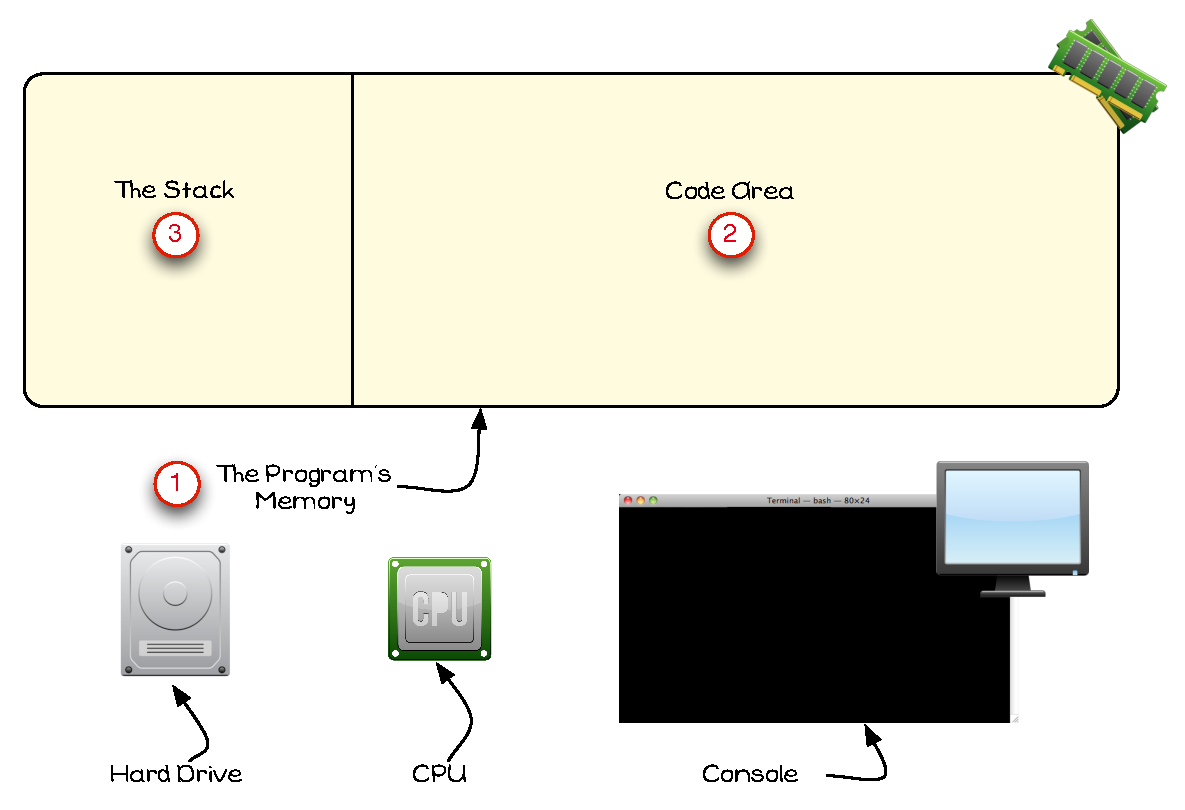
\includegraphics[width=\textwidth]{./topics/program-creation/images/ProgramExecution01} 
   \caption[Program Memory Space]{Operating System prepares memory for the Program}
   \label{fig:program-creation-visualise-helloworld-1}
\end{figure}

\mynote{
\begin{itemize}
  \item In Figure \ref{fig:program-creation-visualise-helloworld-1} the indicated areas show the following:
  \begin{enumerate}
    \item The Operating System allocates memory for the program.
    \item Part of the allocated memory will be designated to store the program's instructions. This can be thought of as the \emph{Code Area}.
    \item Another part of the allocated memory will be set aside to keep track of the current instruction. This area is called the \emph{Stack}.
  \end{enumerate}
\end{itemize}
}

% subsubsection allocating_memory_for_the_program (end)
\clearpage
\subsubsection{Loading the Code} % (fold)
\label{ssub:loading_the_code}

Having allocated the program some memory, and partitioned this space into the \textbf{Stack} and \textbf{Code} area, the Operating System then reads the program's instructions from the executable file and loads these into the Code area. This is illustrated in Figure \ref{fig:program-creation-visualise-helloworld-2}.

\begin{figure}[htbp]
   \centering
   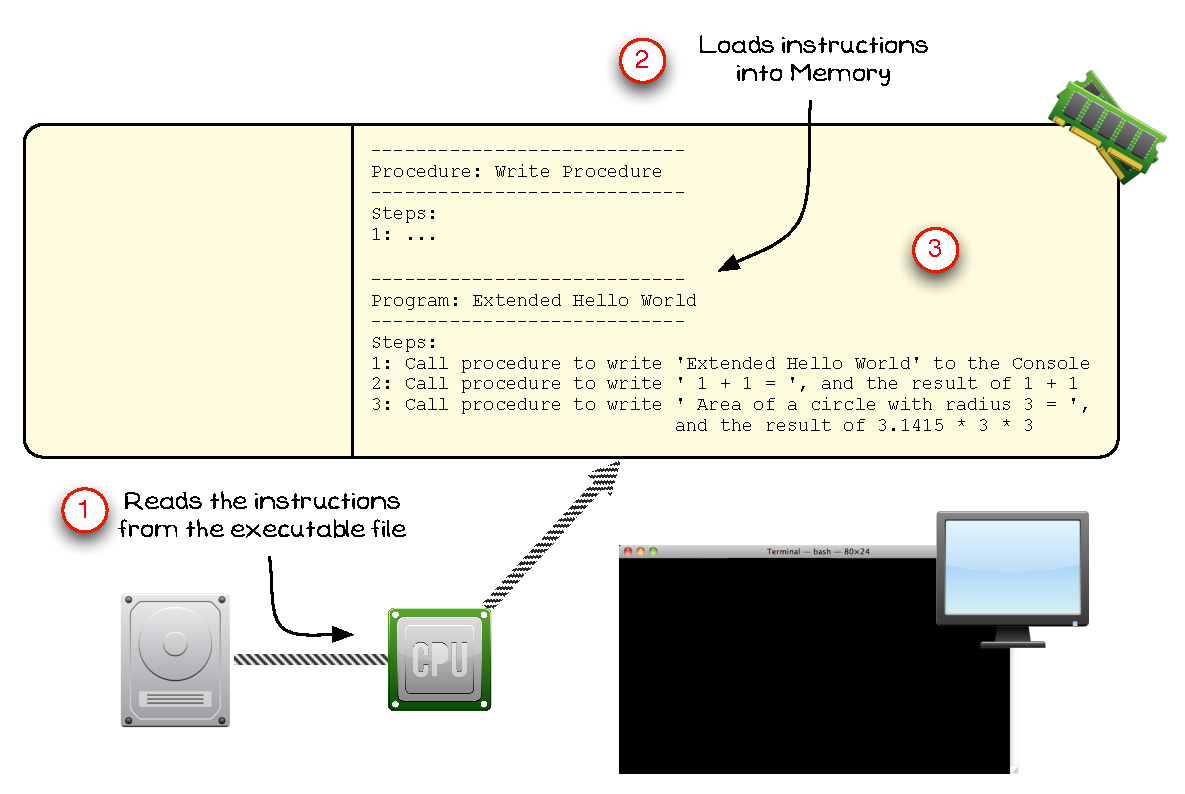
\includegraphics[width=\textwidth]{./topics/program-creation/images/ProgramExecution02} 
   \caption[Code loaded into memory]{The Operating System loads the program's code into memory}
   \label{fig:program-creation-visualise-helloworld-2}
\end{figure}

\mynote {
\begin{itemize}
  \item In Figure \ref{fig:program-creation-visualise-helloworld-2} the indicated areas show the following:
  \begin{enumerate}
    \item The program's instructions are read from the executable file the user launched.
    \item The instructions are stored into the program's memory: into the code area.
    \item When this finishes, all of the program's instructions are loaded into memory. In Figure \ref{fig:program-creation-visualise-helloworld-2} the instructions are shown as the pseudocode from Listing \ref{lst:program-creation-hello-pseudo}. In reality these will be the \emph{machine code} instructions that were saved into the executable file by the compiler.
  \end{enumerate}
  \bigskip
  \item The \emph{Operating System} is a software component that is used to control access to the hardware. In this case the Operating System takes the responsibility for setting up the machine so that it can run the program the user launched.
\end{itemize}
}
% subsubsection loading_the_code (end)

\clearpage
\subsubsection{Setting Up The First Instruction} % (fold)
\label{ssub:setting_up_the_first_instruction}

Now that the code is loaded into memory, the Operating System uses the details saved in the executable file to setup the program's first instruction. This will be loaded onto the Stack, which is responsible for keeping track of the current instruction. The compiler will have used the program's \textbf{entry point} to store these details when the program was compiled. This is shown in Figure \ref{fig:program-creation-visualise-helloworld-3}.

\begin{figure}[htbp]
   \centering
   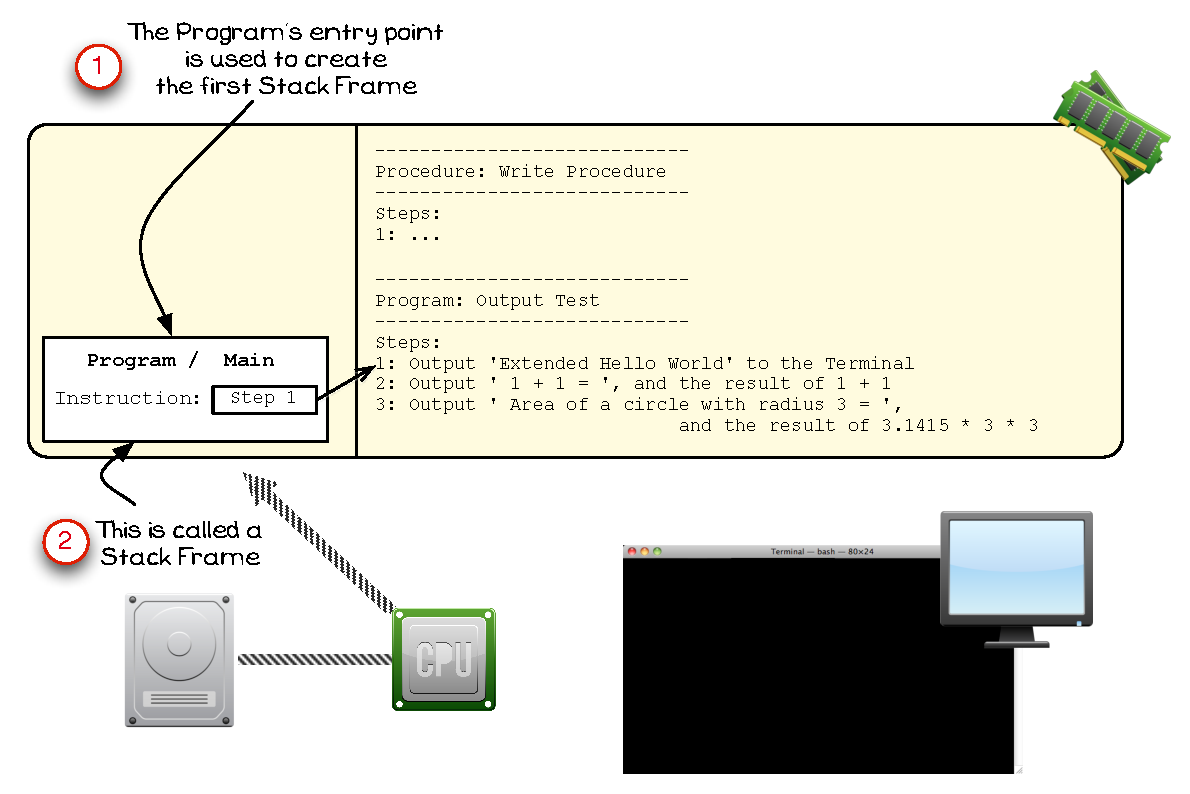
\includegraphics[width=\textwidth]{./topics/program-creation/images/ProgramExecution03} 
   \caption{The current instruction is loaded onto the Stack}
   \label{fig:program-creation-visualise-helloworld-3}
\end{figure}

\mynote {
\begin{itemize}
  \item In Figure \ref{fig:program-creation-visualise-helloworld-3} the indicated areas show the following:
  \begin{enumerate}
    \item The program's instruction is tracked on \emph{The Stack}.
    \item Each Stack Frame keeps a record of the current instruction within a Procedure. This area is called the Stack as the Frames are \emph{stacked} one on top of the other. The one on the top of the \emph{stack} tells the computer which instruction is to be run.
  \end{enumerate}
  \bigskip
  
  \item The Stack keeps track of the current instruction.
  \item The current instruction refers to the code loaded into the Code area.
  \item The compiler will have saved the details for which instruction is first into the executable file.
  \item In your code the program's \textbf{entry point} tells you which instruction will be first.
\end{itemize}
}

% subsubsection setting_up_the_first_instruction (end)

\clearpage
\subsubsection{Running The First Instruction} % (fold)
\label{ssub:running_the_first_instruction}

The Operating System has finally finished loaded the Program, and can now start its instructions running. The CPU uses the \textbf{Current Instruction} that is on the top of the Stack, locates the Code, and runs the instruction. In this case this is a procedure call to a Procedure that writes output to the Terminal. When this instruction completes, the text \emph{Output Test Program} will have appeared on the Terminal for the user to see. The results of this are shown in Figure \ref{fig:program-creation-visualise-helloworld-4}. 

\begin{figure}[htbp]
   \centering
   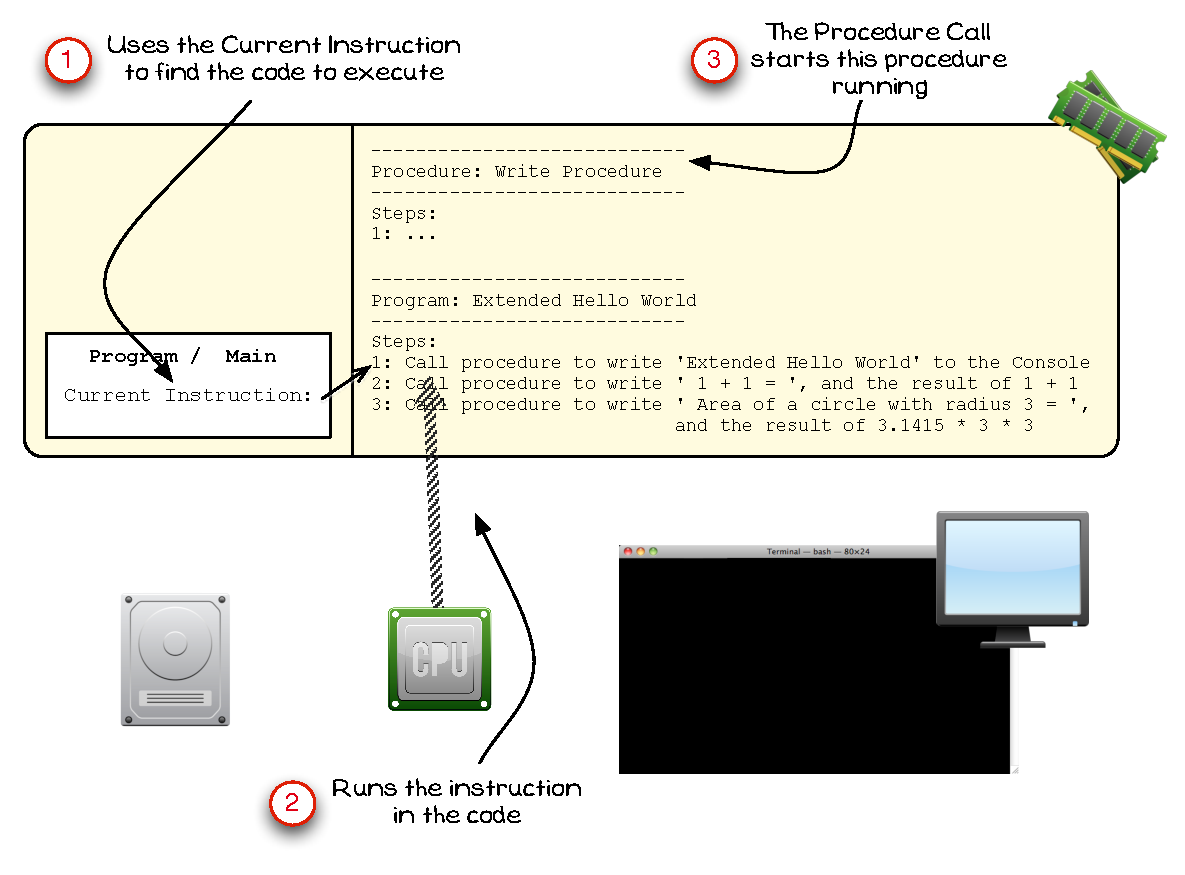
\includegraphics[width=\textwidth]{./topics/program-creation/images/ProgramExecution04} 
   \caption{The Computer runs the first instruction, outputting details to the Terminal}
   \label{fig:program-creation-visualise-helloworld-4}
\end{figure}


\mynote{
\begin{itemize}
  \item In Figure \ref{fig:program-creation-visualise-helloworld-4} the indicated areas show the following:
  \begin{enumerate}
    \item The current instruction is read from the Frame on the top of the Stack.
    \item The Computer runs the instruction from the code loaded into memory.
    \item The instruction is a procedure call, which starts the execution of the Write Procedure.
  \end{enumerate}
  
  \bigskip
  \item The computer runs the code \textbf{one} instruction at a time.
  \item When that instruction is finished it moves onto the next instruction. This is important, and means that are programs run the commands in \textbf{Sequence}.
  \item Writing data to the Terminal takes more than a single instruction, the procedure call gets the Computer to run the instructions in the called Procedure.
\end{itemize}
}

% subsubsection running_the_first_instruction (end)
% subsection starting_a_program (end)

\clearpage
\subsection{Calling the Write Procedure} % (fold)
\label{sub:calling_a_procedure}

At this point the Computer has been instructed to \texttt{Call the Write Procedure}. This procedure\footnote{The \texttt{printf} procedure in C and the \texttt{WriteLn} procedure in Pascal.} will output the data passed to it to the Terminal. In order to do this, the instructions within the called procedure need to be followed.

\subsubsection{Calling Write for the first time} % (fold)
\label{ssub:calling_write_for_the_first_time}

Each Procedure contains instructions that when followed get the Computer to perform a task. The procedure call sets up the Stack so that the instructions within the Write Procedure are executed.

\begin{figure}[htbp]
   \centering
   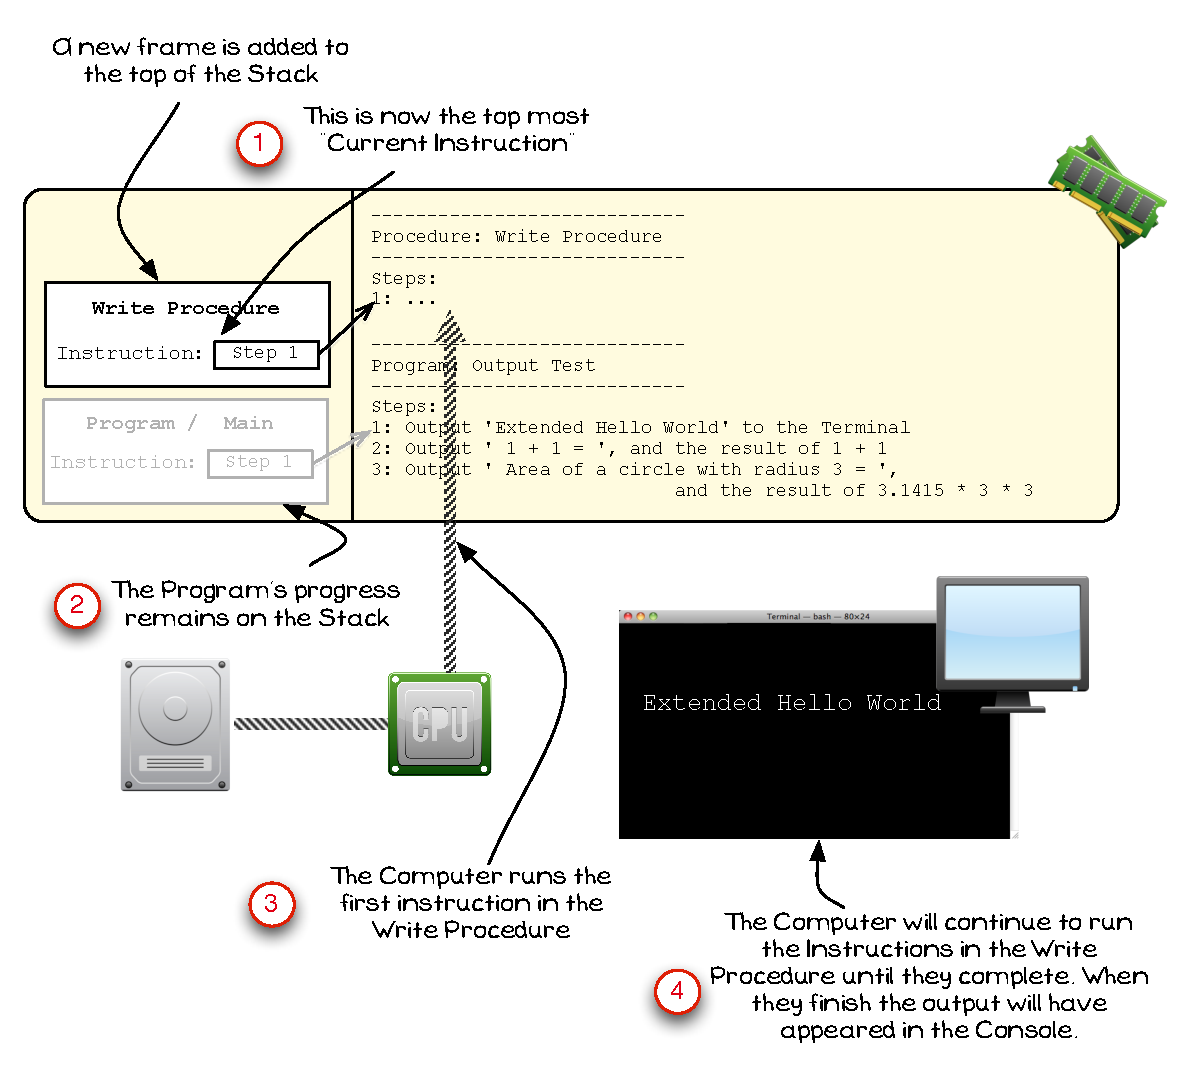
\includegraphics[width=0.9\textwidth]{./topics/program-creation/images/ProgramExecution05} 
   \caption{The Write Procedure is called, and has its instructions executed}
   \label{fig:program-creation-visualise-helloworld-5}
\end{figure}

\mynote{
\begin{itemize}
  \item In Figure \ref{fig:program-creation-visualise-helloworld-5} the indicated areas show the following:
  \begin{enumerate}
    \item A new Frame is added to the Stack for the Write Procedure.
    \item The new Frame appears on top of the Frame that has the program's Current Instruction.
    \item Now the Computer can run the instructions within the Write Procedure.
    \item The instructions are run one at a time until the Write Procedure finishes. At this time the first output will have appeared on the Terminal.
  \end{enumerate}
\end{itemize}
}


% subsubsection calling_write_for_the_first_time (end)
\clearpage
\subsubsection{The Write Procedure Ends} % (fold)
\label{ssub:the_write_procedure_ends}

When the Write Procedure's instructions finish control needs to return to the code that called it, in this case the program's code.

\begin{figure}[htbp]
   \centering
   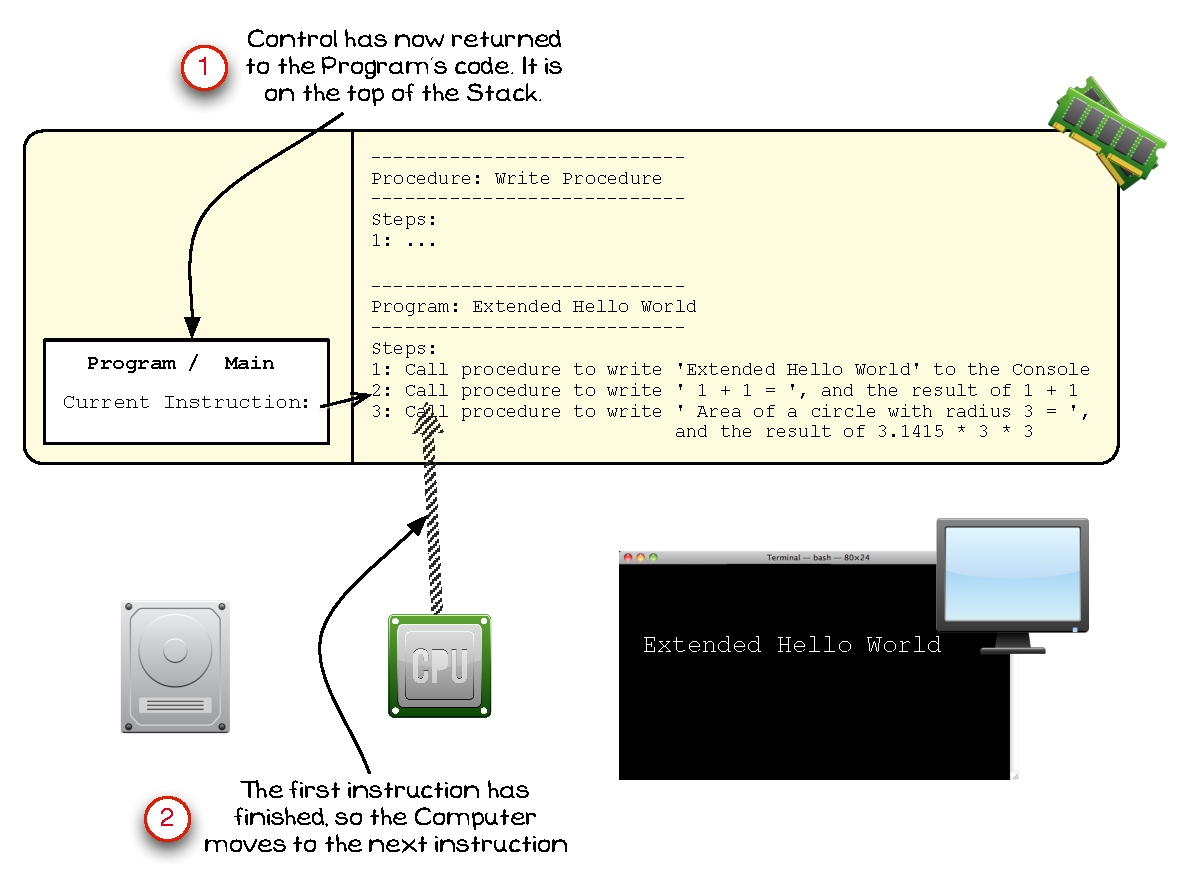
\includegraphics[width=\textwidth]{./topics/program-creation/images/ProgramExecution06} 
   \caption{The Write Procedure is called, and has its instructions executed}
   \label{fig:program-creation-visualise-helloworld-6}
\end{figure}

\mynote{
\begin{itemize}
  \item In Figure \ref{fig:program-creation-visualise-helloworld-6} the indicated areas show the following:
  \begin{enumerate}
    \item When the Write Procedure finishes its Frame is removed from the Stack, and control returns to the program's code.
    \item The first instruction on the program's code has now finished, so the Computer moves to the second instruction.
  \end{enumerate}
\end{itemize}
}

One way to visualise this is to picture the Program, and the Procedure, as a book of instructions. Imagine you are told to follow the instructions in a book. You get the book, place it on a table and read the first instruction which tells you to perform the \emph{Write Procedure}. You leave the original book on the table, and fetch the \emph{Write Procedure} book and place it on top of the book on the table, thereby creating a Stack of books. Now you can follow the instructions, one by one, from the book on top of the Stack. When you finish the last instruction you take the book off the top of the stack and return to the book beneath it. This will enable you to perform the steps within the Procedures without forgetting where you are up to in the earlier code.


% subsubsection the_write_procedure_ends (end)
\clearpage
\subsubsection{The Second Call to Write} % (fold)
\label{ssub:the_second_call_to_write}

The second instruction in the program's code is another call to the Write procedure.

\begin{figure}[htbp]
   \centering
   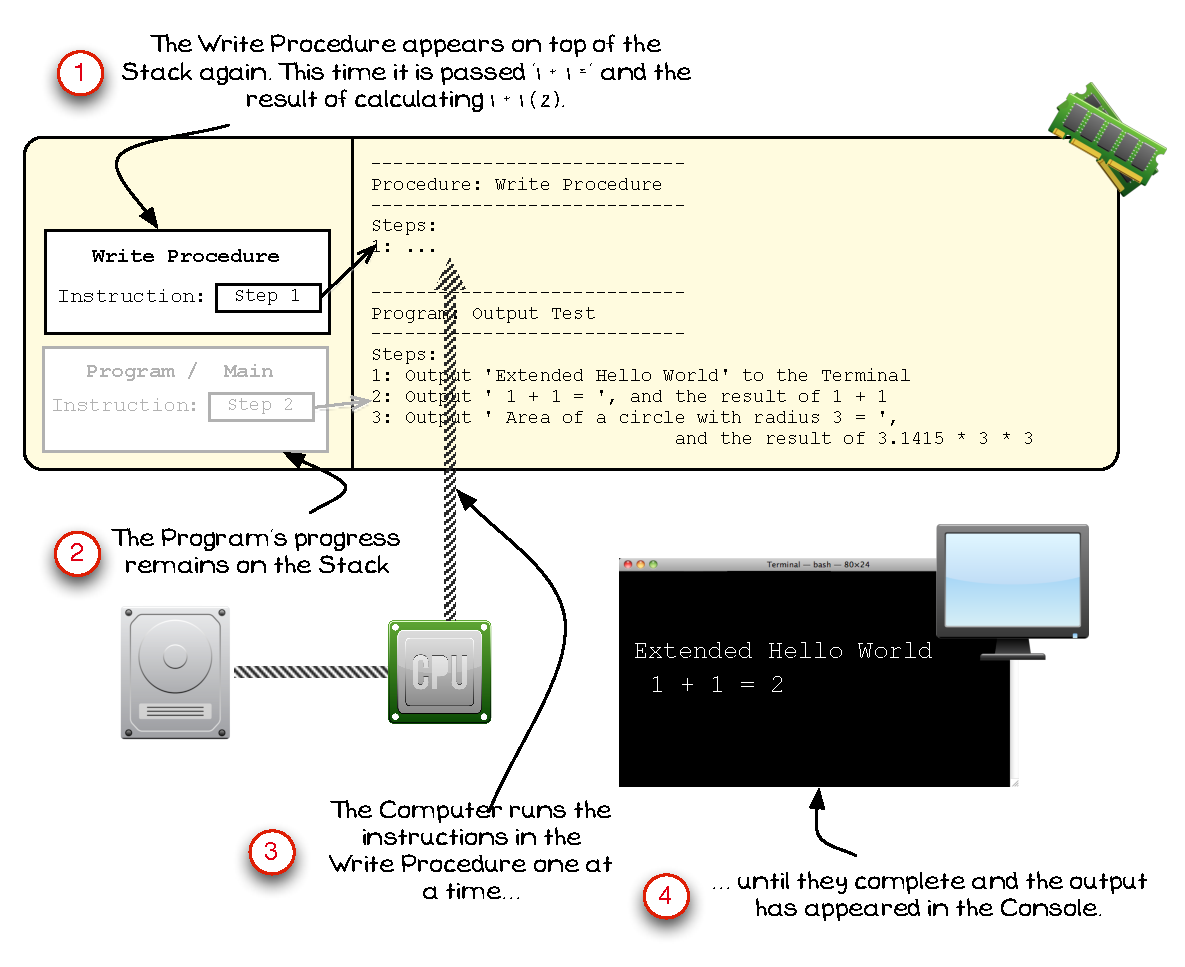
\includegraphics[width=\textwidth]{./topics/program-creation/images/ProgramExecution07} 
   \caption{The Write Procedure is called a second time}
   \label{fig:program-creation-visualise-helloworld-7}
\end{figure}

\mynote{
\begin{itemize}
  \item In Figure \ref{fig:program-creation-visualise-helloworld-7} the indicated areas show the following:
  \begin{enumerate}
    \item A new Frame is created for the Write Procedure. This allows the Computer to keep track of which statement is the current statement within this Procedure.
    \item The program's current instruction remains on the Stack for when the call to the Write procedure finishes.
    \item Each of the instructions in the Write procedure are executed to write the data to the Terminal.
    \item The output text appears on the Terminal.
  \end{enumerate}
\end{itemize}
}

% subsubsection the_second_call_to_write (end)
\clearpage
\subsubsection{The Second Write Call Ends} % (fold)
\label{ssub:the_second_write_call_ends}

When the second call to Write ends control returns to the Program, which moves on to its final instruction.

\begin{figure}[htbp]
   \centering
   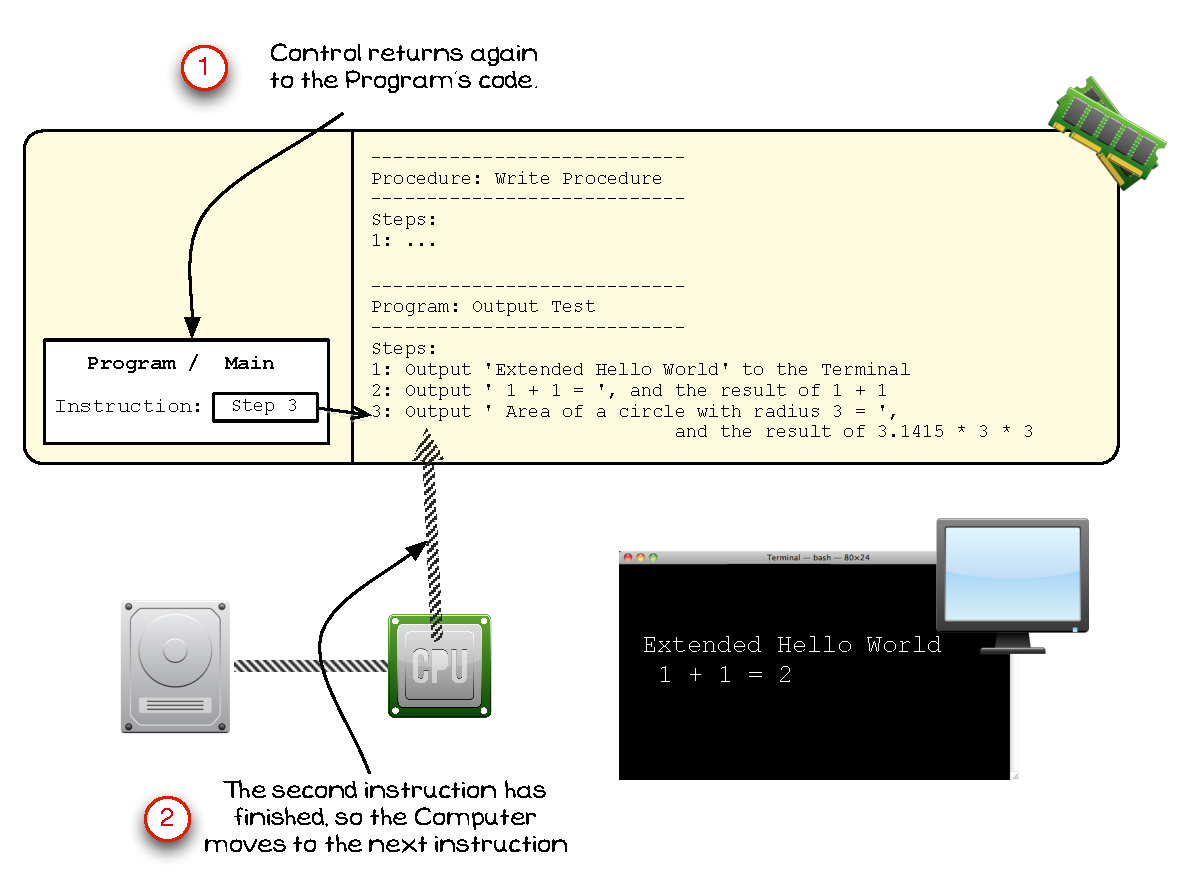
\includegraphics[width=\textwidth]{./topics/program-creation/images/ProgramExecution08} 
   \caption{The second call to the Write Procedure ends, and control returns to the Program}
   \label{fig:program-creation-visualise-helloworld-8}
\end{figure}

\mynote{
\begin{itemize}
  \item In Figure \ref{fig:program-creation-visualise-helloworld-8} the indicated areas show the following:
  \begin{enumerate}
    \item When the second call to the Write Procedure ends control returns to the program's code.
    \item As the second instruction has now finished the Computer moves to the third, and final, instruction in the program.
  \end{enumerate}
\end{itemize}
}

% subsubsection the_second_write_call_ends (end)
\clearpage
\subsubsection{The Third Call to Write} % (fold)
\label{ssub:third_call_to_write}

The final instruction in the program is a third call to the Write Procedure. 

\begin{figure}[htbp]
   \centering
   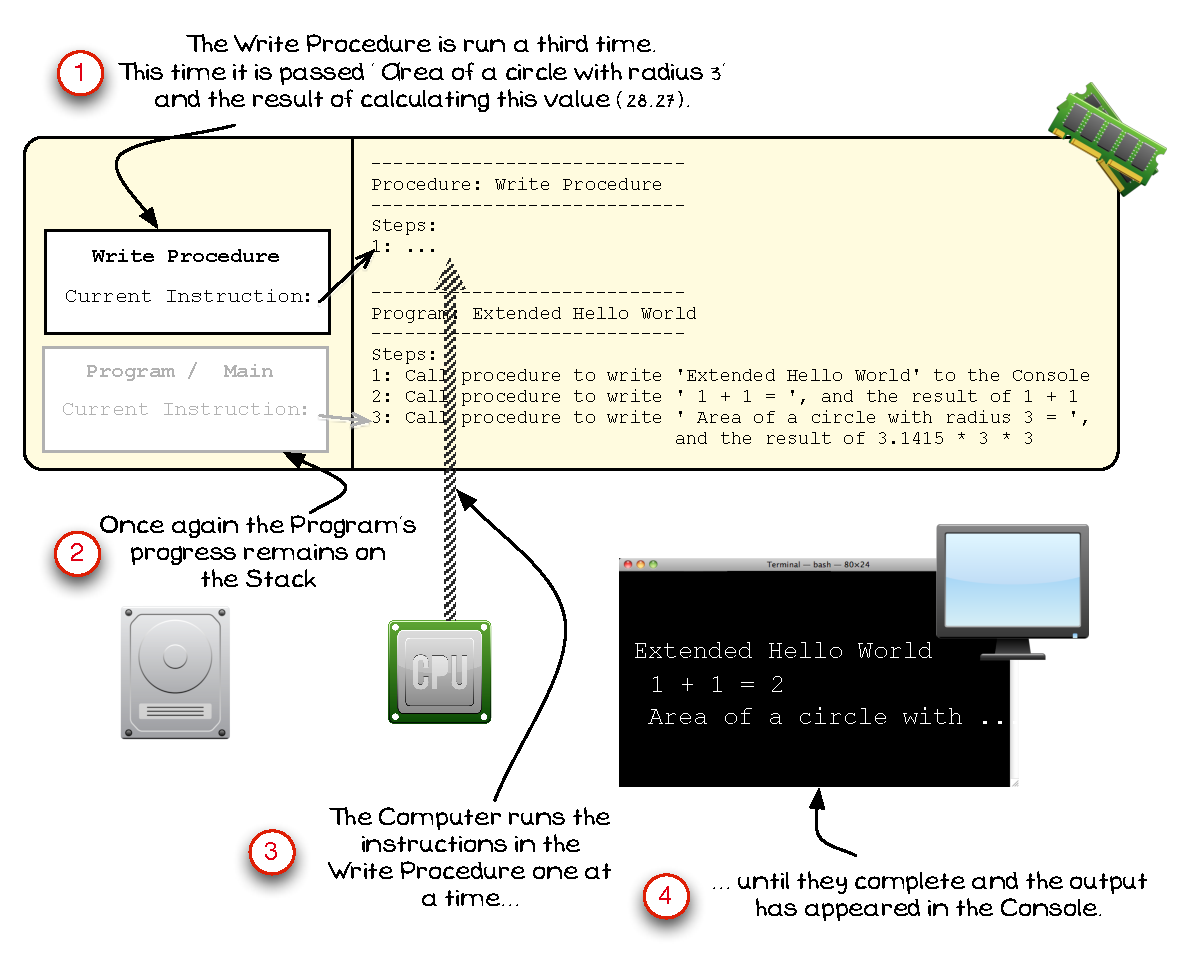
\includegraphics[width=\textwidth]{./topics/program-creation/images/ProgramExecution09} 
   \caption{The Write Procedure is called a third can final time}
   \label{fig:program-creation-visualise-helloworld-9}
\end{figure}

\mynote{
\begin{itemize}
  \item In Figure \ref{fig:program-creation-visualise-helloworld-9} the indicated areas show the following:
  \begin{enumerate}
    \item Once again, a Stack Frame is created to keep track of the progress within the Write Procedure.
    \item The program's current instruction remains on the Stack so that the Computer can return to it when the Write Procedure ends.
    \item Each of the instructions in the Write Procedure are executed.
    \item The Write Procedure writes the data passed to it to the Terminal.
  \end{enumerate}
\end{itemize}
}

% subsubsection third_call_to_write (end)
\clearpage
\subsubsection{The Program Ends} % (fold)
\label{ssub:program_ends}

When the last instruction in the Write Procedure finishes control return back to the Program, which has no more instructions. This means that the program has finished.

\begin{figure}[htbp]
   \centering
   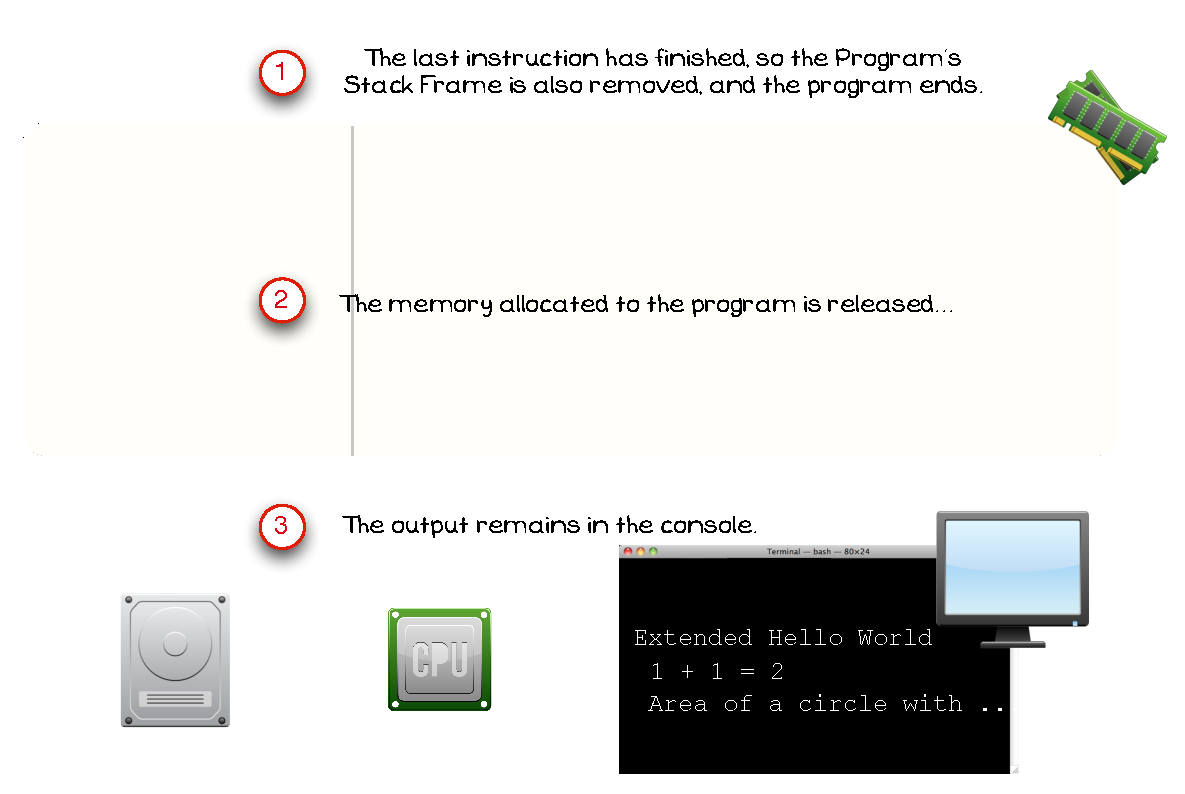
\includegraphics[width=\textwidth]{./topics/program-creation/images/ProgramExecution10} 
   \caption{The Write Procedure ends, then the program ends}
   \label{fig:program-creation-visualise-helloworld-10}
\end{figure}

\mynote{
\begin{itemize}
  \item In Figure \ref{fig:program-creation-visualise-helloworld-10} the indicated areas show the following:
  \begin{enumerate}
    \item The Write Procedure has finished its instructions, and so it ends. This was also the last instruction in the program's code, so it also ends. This tells the Operating System that Program has finished.
    \item The Operating System releases the memory used by the program so that it can be use by other programs.
    \item All of this will have happened in an instant, and after the program has finished all that remains is the output in the Terminal.
  \end{enumerate}
\end{itemize}
}

% subsubsection program_ends (end)

% subsection calling_a_procedure (end)
\clearpage
\subsection{Summary} % (fold)
\label{sub:program_creation_visualise_summary}

In this section you have seen the actions that occur behind the scenes when your program is executed. The most important aspects are the fact that the instructions run one at a time in \textbf{sequence}, and that a procedure call results in the instructions within the Procedure running until they end. Its also important to remember that the instructions within the Procedure must finish before control returns to where the call was made.

\bigskip

\mynote{
\begin{itemize}
  \item A Program is a sequence of instructions.
  \item These instructions are organised into Procedures that can be called. 
  \item The program's instructions are loaded into memory when the program is launched.
  \item Instructions are run one at a time.
  \item The Stack is used to keep track of the current instruction.
  \item When the program starts a Frame is added to the Stack to set the entry point as the first instruction.
  \item When a Procedure is called, a Frame is added to the Stack to keep track of its current instruction. 
\end{itemize}
}

% subsection summary (end)

% section understanding_program_execution (end)

% ====================
% = Examples Section =
% ====================
\clearpage
\section{Program Creation Examples} % (fold)
\label{sec:program_creation_examples}

\subsection{Seven Times Table} % (fold)
\label{sub:seven_times_table}

This program prints out the seven times table from 1 x 7 to 10 x 7. The description of the program is in Table \ref{tbl:program-creation-times-table}, the pseudocode in Listing \ref{lst:program-creation-seven-times-pseudo}, the C code in Listing \ref{lst:program-creation-seven-times-c}, and the Pascal code in Listing \ref{lst:program-creation-seven-times-pas}.

\begin{table}[h]
\centering
\begin{tabular}{l|p{10cm}}
  \hline
  \multicolumn{2}{c}{\textbf{Program Description}} \\
  \hline
  \textbf{Name} & \emph{Seven Times Table} \\
  \\
  \textbf{Description} & Displays the Seven Times Table from 1 x 7 to 10 x 7. \\
  \hline
\end{tabular}
\caption{Description of the Seven Times Table program}
\label{tbl:program-creation-times-table}
\end{table}

\pseudocode{lst:program-creation-seven-times-pseudo}{Pseudocode for Seven Times Table program.}{./topics/program-creation/examples/seven-times.txt}

\clearpage

\csection{\ccode{lst:program-creation-seven-times-c}{C Seven Times Table}{topics/program-creation/examples/seven_times.c}}
\passection{\pascode{lst:program-creation-seven-times-pas}{Pascal Seven Times Table}{topics/program-creation/examples/SevenTimesTable.pas}}

% subsection times_table (end)
\clearpage
\subsection{Circle Area} % (fold)
\label{sub:circle_area}

This program prints out the area of circles with different radius. The description of the program is in Table \ref{tbl:program-creation-circle-area}, the pseudocode in Listing \ref{lst:program-creation-circle-areas-pseudo}, the C code in Listing \ref{lst:program-creation-circle-areas-c}, and the Pascal code in Listing \ref{lst:program-creation-circle-areas-pas}.

\begin{table}[h]
\centering
\begin{tabular}{l|p{10cm}}
  \hline
  \multicolumn{2}{c}{\textbf{Program Description}} \\
  \hline
  \textbf{Name} & \emph{Circle Areas} \\
  \\
  \textbf{Description} & Displays the Circle Areas for circles with radius from 1.0 to 5.0 with increments of 0.5. \\
  \hline
\end{tabular}
\caption{Description of the Circle Areas program}
\label{tbl:program-creation-circle-area}
\end{table}

\pseudocode{lst:program-creation-circle-areas-pseudo}{Pseudocode for Circle Area program.}{./topics/program-creation/examples/circle_areas.txt}

\clearpage

\csection{\ccode{lst:program-creation-circle-areas-c}{C Circle Areas}{topics/program-creation/examples/circle_areas.c}}
\passection{\pascode{lst:program-creation-circle-areas-pas}{Pascal Circle Areas}{topics/program-creation/examples/CircleAreas.pas}}

% subsection circle_area (end)
\clearpage
\subsection{Shape Drawing} % (fold)
\label{sub:shape_drawing}

This program draws some shapes to the screen using the \textbf{SwinGame} Software Development Kit (SDK). The SwinGame SDK is a library that provides a number of reusable code artefacts that you can use to create 2D games. This SDK is available for both C and Pascal, and work on Linux, Mac, and Windows.

The description of the program is in Table \ref{tbl:program-creation-shape-drawing}, the pseudocode in Listing \ref{lst:program-creation-shape-drawing-pseudo}, the C code in Listing \ref{lst:program-creation-shape-drawing-c}, and the Pascal code in Listing \ref{lst:program-creation-shape-drawing-pas}.

\begin{table}[h]
\centering
\begin{tabular}{l|p{10cm}}
  \hline
  \multicolumn{2}{c}{\textbf{Program Description}} \\
  \hline
  \textbf{Name} & \emph{Shape Drawing} \\
  \\
  \textbf{Description} & Draws a number of shapes to the screen using SwinGame. \\
  \hline
\end{tabular}
\caption{Description of the Shape Drawing program}
\label{tbl:program-creation-shape-drawing}
\end{table}

\pseudocode{lst:program-creation-shape-drawing-pseudo}{Pseudocode for Shape Drawing program.}{./topics/program-creation/examples/shape_drawing.txt}

The Lines from the program will do the following:
\begin{itemize}
  \item \textbf{\texttt{OpenGraphicsWindow}} opens a Window with the title `Shape Drawing' that is 800 pixels wide by 600 pixels high.
  \item \textbf{\texttt{ClearScreen}} clears the screen to black.
  \item \textbf{\texttt{FillRectangle}} uses the color, the x, y location, and width and height to fill a rectangle.
  \item \textbf{\texttt{RefreshScreen}} updates the screen to show what has been drawn. All SwinGame drawing is done offscreen, and only drawn to the screen when RefreshScreen is called.
  \item \textbf{\texttt{Delay}} pauses the program for a number of milliseconds, so 500 will wait for half a second.
  \item \textbf{\texttt{FillCircle}} uses the color, given x, y location and radius to fill a circle.
  \item \textbf{\texttt{FillTriangle}} fills a triangle with the given x, y points (6 values for 3 points).
\end{itemize}

\clearpage

\csection{\ccode{lst:program-creation-shape-drawing-c}{C Shape Drawing Code}{topics/program-creation/examples/shape_drawing.c}}

The SwinGame procedure for C are named using the standard C naming scheme. The names are:
\begin{itemize}
  \item \textbf{\texttt{open\_graphics\_window}} opens a Window with the title `Shape Drawing' that is 800 pixels wide by 600 pixels high.
  \item \textbf{\texttt{load\_default\_colors}} loads default colors for use in your code.
  \item \textbf{\texttt{clear\_screen}} clears the screen to black.
  \item \textbf{\texttt{fill\_rectangle}} uses the color, the x, y location, and width and height to fill a rectangle.
  \item \textbf{\texttt{refresh\_screen}} updates the screen to show what has been drawn. All SwinGame drawing is done offscreen, and only drawn to the screen when RefreshScreen is called.
  \item \textbf{\texttt{delay}} pauses the program for a number of milliseconds, so 500 will wait for half a second.
  \item \textbf{\texttt{fill\_circle}} uses the color, given x, y location and radius to fill a circle.
  \item \textbf{\texttt{fill\_triangle}} fills a triangle with the given x, y points (6 values for 3 points).
\end{itemize}


\clearpage

\passection{\pascode{lst:program-creation-shape-drawing-pas}{Pascal Shape Drawing Code}{topics/program-creation/examples/ShapeDrawing.pas}}


% subsection shape_drawing (end)

% section program_creation_examples (end)

% =============
% = Exercises =
% =============
\clearpage
\section{Program Creation Exercises} % (fold)
\label{sec:program_creation_exercises}

\begin{enumerate}
  \item Write a program that prints the 73 times table from 1 * 73 to 10 * 73.
  \begin{itemize}
    \item Draw up a outline of the program
    \item Write pseudocode for the program's instructions
    \item Convert your pseudocode to either C or Pascal
    \item Compile and Run your program, and check that the values are correctly calculated
  \end{itemize}
  
  \item Write a program that prints the powers\footnote{In the code you will need to calculate these manually using times ($2^1$ = 2, $2^2$ = 2*2, $2^3$ = 2*2*2, etc.)} of 2 from $2^1$ to $2^8$.
  \begin{itemize}
    \item Draw up a outline of the program
    \item Write pseudocode for the program's instructions
    \item Convert your pseudocode to either C or Pascal
    \item Compile and Run your program, and check that the values are correctly calculated
  \end{itemize}
  
  
  \item Write a program that prints a table that shows calculations related to circles. This should output the  radius, circle area, diameter, and circumference.
  \begin{itemize}
    \item Find the necessary calculations and then draw up a outline of the program
    \item Write pseudocode for the program's instructions
    \item Convert your pseudocode to either C or Pascal
    \item Compile and Run your program, and check that the values are correctly calculated
  \end{itemize}
  
  \item Write a program that draws a face on the screen using SwinGame.
  \begin{itemize}
    \item Draw up an outline of the program. Work out the coordinates of the circles for the face, circles. Determine three points of the triangle for the mouth.
    \item Write up the pseudocode for the program's instructions. Remember to use the \texttt{RefreshScreen} and \texttt{Delay} procedures to see the results.
    \item Convert your pseudocode to either C or Pascal
    \item Compile and Run your program, and check that the values are correctly calculated
  \end{itemize}
\end{enumerate}

% section program_creation_exercises (end)

% ===================
% = Project Section =
% ===================
\clearpage
\section{Program Creation Project} % (fold)
\label{sec:program_creation_project}

% section program_creation_project (end)

% chapter program_creation (end)